\section{Deep Learning}\label{sec:deep_learning}
\acrfull{ai}, \acrfull{ml}, and deep learning are terms often used interchangeably and to describe a wide range of topics. The beginning of this section tries to clarify the meaning of these terms in the context of this work before discussing the topic of deep learning in more detail.

\acrshort{ai} is the broadest of the three topics and encompasses the others~\cite{Goodfellow:2016:DNN}. 
%Fig 1.4
While it lacks an agreed-upon definition, the term broadly describes the research dedicated to creating machines that enact some form of intelligence \cite{nilsson:2009}. However, this only shifts the burden of definition to the term ``intelligence''. In his excellent book on the history of \acrshort{ai} Nilsson describes intelligence as the ``quality that enables an entity to function appropriately and with foresight in its environment'' \cite{nilsson:2009}. Taking these definitions as a basis, \acrshort{ai} research tries to create algorithms or machines that make decisions based on their environment to maximize their chance of success to achieve some goal.

\acrshort{ml} is part of the research field on \acrshort{ai} and aims to create algorithms that extract general features from example data. These learned features are then to be used to make predictions about samples that were not part of the example data. It specifically requires algorithms to improve based on past experiences~\cite{Goodfellow:2016:DNN}. 
%page 1
Usually, a general purpose framework is adapted to specific problems only through a prior training phase, where the algorithm is exposed to example data. This means that the learning algorithm does not have to be changed to adapt to different data.

An example for a class of \acrshort{ai} algorithms that do not fall under the category of \acrshort{ml} algorithms are knowledge based approaches. These try to encode knowledge in a formal language and infer decisions by querying the resulting database.~\cite{Goodfellow:2016:DNN}. 
%page 2
The Cyc project is one of the most well known approaches to a knowledge based \acrshort{ai} and makes use of the CycL language~\cite{Lenat:1989aaa}. However, creating a database that is both suitably large and complex is very labor intensive and often more fragile than utilizing \acrshort{ml} algorithms. For these reasons \acrshort{ml} is currently the most widespread approach to \acrshort{ai}.

Deep learning refers to \acrshort{ml} algorithms which utilize a specific kind of framework; deep neural networks (\acrshort{nn}s). While the concept of \acrshort{nn}s will be introduced in detail below, in short they are directed graphs that apply simple functions at every node, where the weights of the edges are optimized during the training phase based on the example data. These graphs can be structured into layers and a \acrshort{nn} is called deep, when the network is composed of many subsequent layers~\cite{Goodfellow:2016:DNN}.

Besides deep learning, there are many other kinds of \acrshort{ml} algorithms. Some examples include random forests~\cite{Ho:1995aaa}, support vector machines (\acrshort{svm}s) \cite{Boser:1992aaa}, and Gaussian process regression. Even simple regression algorithms, like linear regression, can be seen as a kind of \acrshort{ml} algorithms~\cite{Geron:2017aaa}. 
%page XV
For a short overview of these different types see for instance chapter 1 and for a more detailed discussion chapters 5 to 7 of \cite{Geron:2017aaa}.

All \acrshort{ml} algorithms can broadly be classified into three categories based on the~\emph{training} mechanism, where training is the process of improving the algorithm based on example data. These three classes are \emph{supervised learning}, \emph{unsupervised learning}, and \emph{reinforcement learning}~\cite{Goodfellow:2016:DNN, Ghahramani:2004}. In supervised learning tasks the desired output $y$ -- often called \emph{label} or \emph{target} -- for example data $x$ is known~\cite{Geron:2017aaa} and the algorithm tries to approximate the conditional probability distribution $p\lr{y \given x}$~\cite{Goodfellow:2016:DNN}. 
%page 8 and page 103
Regression algorithms are a good example for supervised learning. In unsupervised learning only the example data $x$ is known and the \acrshort{ml} algorithm is tasked with finding the underlying probability distribution $p\lr{x}$~\cite{Goodfellow:2016:DNN}. 
%page 103
Many clustering algorithms are a prime example for unsupervised learning. Reinforcement learning is completely detached from the previous two classes. Here the algorithm observes the state of its environment and has to decide on an action it wants to take. It is then rewarded or penalized based on the action it has chosen~\cite{Geron:2017aaa,sutton:2018}. 
%page 8
The algorithm learns by trial and error, without human intervention. This kind of learning is especially popular in the field of robotics and computer games~\cite{Goodfellow:2016:DNN,Finn:2015aaa,Sallab:2017,Mnih:2015aaa,openai:2019}.
%page 25
The above mentioned classifications of algorithms are by no means rigid. A single algorithm may also be trained by a combination of the above mentioned strategies. There are also other means of classifying \acrshort{ml} algorithms into different categories~\cite{Geron:2017aaa}.
%page 8

Today \acrshort{ml} algorithms are used anywhere from recommendation systems in the entertainment industry~\cite{Steck:2021aaa} to advanced medical diagnostics~\cite{Esteva:2019aaa}. Especially \acrshort{nn}s have gained a lot of traction in recent years and improved state-of-the-art performance for \acrshort{ml} algorithms for a wide variety of tasks such as image recognition \cite{krizhevsky:2012, Szegedy:2015, Russakovsky:2015aaa}, autonomous driving \cite{Sallab:2017}, playing board- \cite{Silver:2016} and computer-games \cite{openai:2019}, speech recognition \cite{Hinton:2012}, or audio synthesis \cite{Oord:2016wav}. \acrshort{ml} algorithms have also been applied in many scientific fields~\cite{Deiana:2021niw}, some of which are the prediction of protein structure used in pharmaceutical studies~\cite{Alquraishi:2021aaa, Jumper:2021aaa}, improvements to material composition and synthesis~\cite{Butler:2018aaa}, and event reconstruction at the Large Hadron Collider~\cite{Gray:2020mcm}. Machine learning has also been explored as an option for many tasks in \acrshort{gw} data analysis and \acrshort{gw} astronomy and an overview is given in \autoref{sec:ml-gw-hist}.

This work considers only neural networks as a means of machine learning. For this reason the basic concepts as well as a few advanced techniques will be briefly introduced in the following subsections. For a more thorough introduction I recommend \cite{Goodfellow:2016:DNN} for a deep dive into the topic, \cite{Geron:2017aaa} for a more applied approach, and \cite{Nielsen:2015:DNN} for a quick and easy to understand overview.

\subsection{Neural Networks}\label{sec:nn}
The start of the research on neural networks based on the theory of computation and mathematics can be traced back to a study conducted by McCulloch and Pitts in 1943~\cite{McCulloch:1943}. They tried to come up with a model description of the human brain, where they modeled neurons by utilizing propositional logic. By making the simplifying assumptions that neurons have an arbitrary number of binary inputs, a single binary output that is one (i.e. ``fires'') only if a pre-defined number of inputs is active, and that individual inputs may prevent any output, they were able to build all logic gates and combine them to do complex computations~\cite{Piccinini:2004}. While the original work exclusively used propositional logic, their idea of the neuron can suggestively be expressed by the functional form
\begin{equation}\label{eq:neuron-pitts}
n: {\left\{0,1\right\}}^m\times{\left\{-1,1\right\}}^m\times\mathbb{Z} \to\left\{0,1\right\};\ \lr{\vec{x}, \vec{w}, b} \mapsto H\lr{\vec{x}\cdot\vec{w} + b},
\end{equation}
where $\vec{x}$ are the inputs to the neuron, $\vec{w}$ are known as the weights, $b$ is known as the bias, ans $H$ is the Heaviside function. See \autoref{fig:heavyside_neuron} for a depiction. This definition of the neuron is not equivalent to the idea proposed by McCulloch and Pitts but conveys the central findings of their study and leads to a more coherent picture of subsequent developments.

\begin{figure}
	\centering
	\begin{tikzpicture}[
neuron/.style={minimum size=0.75cm, circle, draw},
heavyside/.style={path picture={
	\pgfpointdiff{\pgfpointanchor{path picture bounding box}{north east}}%
        {\pgfpointanchor{path picture bounding box}{south west}}
      \pgfgetlastxy\x\y
      % Scale the x and y vectors so that the range
      % -1 to 1 is slightly shorter than the size of the node
      \tikzset{x=\x*.25, y=\y*.25}
	\draw (-1,-1) -- (0, -1) -- (0, 1) -- (1, 1);
}}
]

\node[neuron, heavyside] (n) {};

\node (z) [below=0.1cm of n] {$z = \vec{w}\cdot\vec{x}+b$};
\node (x_1) [left=1.5cm of n] {$x_1$};
\node (x_0) [above=0.5cm of x_1] {$x_0$};
\node (x_2) [below=0.5cm of x_1] {$x_2$};
\node (a) [right=1.5cm of n] {$H\lr{z}$};

\draw[->, shorten >= 2pt] (x_0) -- (n) node[midway, above] {$w_0$};
\draw[->, shorten >= 2pt] (x_1) -- (n) node[midway, above] {$w_1$};
\draw[->, shorten >= 2pt] (x_2) -- (n) node[midway, above] {$w_2$};

\draw[->, shorten >= 2pt] (n) -- (a);

\end{tikzpicture}
	\caption[McCulloch-Pitts-neuron]{Depiction of the neuron defined in \eqref{eq:neuron-pitts}. The inputs $x_0, x_1, x_2$ are either $0$ or $1$. The weights $w_0, w_1, w_2$ are either $-1$ or $1$. The bias $b$ is a whole number. $H$ is the Heaviside function.}\label{fig:heavyside_neuron}
\end{figure}

To form basic logic gates, values for the parameters $\vec{w}$ and $b$ have to be chosen. The ''and''-operation $A\land B$ is obtained by setting $\vec{w}=\lr{1, 1}^T,\ b=-1$, whereas the ''not''-operation $\neg A$ can be represented by $w=-1,\ b=1$. These simple gates can then be connected to form complex computational graphs and compute any computable function. However, notice that the parameters of these networks have to be hand-picked.

In 1957 Rosenblatt introduced the Perceptron~\cite{rosenblatt:1958}. Instead of restricting individual neurons to have binary inputs and discrete weights, he allowed all arguments to be real numbers
\begin{equation}\label{eq:neuron-rosenblatt}
n: \R^m\times \R^m\times \R \to \left\{0,1\right\};\ \lr{\vec{x}, \vec{w}, b}\mapsto H\lr{\vec{w}\cdot\vec{x} + b}.
\end{equation}
More importantly, however, he proposed an algorithm based on the Hebbian principal that allowed the parameters of the network to be optimized from example data. The Hebbian principal states that directly connected neurons that often fire together form stronger bonds; ''Neurons that fire together, wire together.''~\cite{Geron:2017aaa} The Perceptron is a collection of these neurons, where every neuron is connected to all inputs. The number of binary outputs, therefore, is equivalent to the number of neurons in the Perceptron. The left panel of \autoref{fig:mlp} shows an example of a perceptron. 

\begin{figure}
	\centering
	\begin{tikzpicture}[
neuron/.style={minimum size=0.75cm, circle, draw},
heavyside/.style={path picture={
	\pgfpointdiff{\pgfpointanchor{path picture bounding box}{north east}}%
        {\pgfpointanchor{path picture bounding box}{south west}}
      \pgfgetlastxy\x\y
      % Scale the x and y vectors so that the range
      % -1 to 1 is slightly shorter than the size of the node
      \tikzset{x=\x*.25, y=\y*.25}
	\draw (-1,-1) -- (0, -1) -- (0, 1) -- (1, 1);
}}
]
\begin{scope}[on grid,node distance=0.5cm]
	% PERCEPTRON
	% Inputs of Perceptron
	\node (x_0) {$x_0$};
	\node (x_1) [below=1cm of x_0] {$x_1$};
	
	% Nodes of Perceptron
	\node[neuron, heavyside] (mlp10) [above right=0.5cm and 1.5cm of x_0] {};
	\node[neuron, heavyside] (mlp11) [below right=0.5cm and 1.5cm of x_0] {};
	\node[neuron, heavyside] (mlp12) [below right=0.5cm and 1.5cm of x_1] {};
	
	% Connections of Perceptron
	\draw[->, shorten >= 2pt] (x_0.east) -- (mlp10);
	\draw[->, shorten >= 2pt] (x_0.east) -- (mlp11);
	\draw[->, shorten >= 2pt] (x_0.east) -- (mlp12);
	
	\draw[->, shorten >= 2pt] (x_1.east) -- (mlp10);
	\draw[->, shorten >= 2pt] (x_1.east) -- (mlp11);
	\draw[->, shorten >= 2pt] (x_1.east) -- (mlp12);
	
	
	% Splitting figure
	\node (a) [above left=0.5cm and 0.5cm of x_0] {(a)};

	\node (ht) [above right=0.25cm and 1cm of mlp10] {};
	\node (hb) [below right=0.25cm and 1cm of mlp12] {};
	
	%\draw[] (ht) -- (hb);
	
	\node (helper1) [right=1cm of ht] {};
	\node (b) at (a -| helper1) {(b)};
	
	
	% MLP
	% Inputs of MLP
	\node (helper2) [right=0.5cm of b] {};
	\node (x_0m) at (x_0 -| helper2) {$x_0$};
	\node (x_1m) [below=1cm of x_0m] {$x_1$};
	
	% MLP layer 1
	\node[neuron, heavyside] (mlp210) [right=1.5cm of x_0m] {};
	\node[neuron, heavyside] (mlp211) [right=1.5cm of x_1m] {};
	
	% MLP layer 2
	\node[neuron, heavyside] (mlp220) [below right=0.5cm and 1.5cm of mlp210] {};
	
	%Connections of MLP
	\draw[->, shorten >= 2pt] (x_0m.east) -- (mlp210);
	\draw[->, shorten >= 2pt] (x_0m.east) -- (mlp211);
	
	\draw[->, shorten >= 2pt] (x_1m.east) -- (mlp210);
	\draw[->, shorten >= 2pt] (x_1m.east) -- (mlp211);
	
	\draw[->, shorten >= 2pt] (mlp210.east) -- (mlp220);
	
	\draw[->, shorten >= 2pt] (mlp211.east) -- (mlp220);
\end{scope}
\end{tikzpicture}
	\caption[Perceptron and Multi-Layer Perceptron]{An example of a perceptron (a) and a \acrshort{mlp} (b). The arrows indicate connections between the input vector $\vec{x}=\lr{x_0, x_1}^T$ and the individual neurons, where each connection is assign a weight. The step inside each neuron represent the Heaviside function that is applied to the weighted sum of the inputs.}\label{fig:mlp}
\end{figure}

During training the output of the Perceptron is compared to the target value. If the predicted output of any neuron does not match the target value, the weights connected to the inputs that would have pushed the output to its correct state are increased~\cite{Geron:2017aaa}. The actual change applied to the weight connecting input $i$ with output neuron $j$ is given by
\begin{equation}\label{eq:rosenblatt-gradient}
dw_{ij}=\eta \lr{y_j-\hat{y}_j}x_i.
\end{equation}
Here $y_j$ is the $j$-th target output, $\hat{y}_j$ is the corresponding predicted output, $x_i$ is the $i$-th input, and $\eta$ is a special parameter called the \emph{learning rate}~\cite{Geron:2017aaa}. Notice that in a Perceptron the neurons are only connected to the inputs and not other neurons.

Although the Perceptron had great success at the time, it was quickly shown that the design had its limitations. One of the greatest criticisms was the inability to represent the XOR-gate, i.e. there exists no Perceptron such that $n\lr{\lr{0,0}, \vec{w}, b}=0,\ n\lr{\lr{0,1}, \vec{w}, b}=1,\ n\lr{\lr{1,0}, \vec{w}, b}=1$, and $n\lr{\lr{1,1}, \vec{w}, b}=0$~\cite{Goodfellow:2016:DNN}. To resolve this issue, the outputs of a first set of neurons have to be used as input to a subsequent neuron. Connecting multiple neurons in succession was hence called a multi-layer Perceptron (\acrshort{mlp}) and the name is still sometimes used today to refer to deep \acrshort{nn}s. Panel (b) of \autoref{fig:mlp} shows a simple \acrshort{mlp} that can represent an XOR-gate, when the weights and biases are chosen correctly.

The \acrshort{mlp} demonstrates that a greater depth of the network, i.e. a greater number of neurons between the input and output, can allow the network to represent more complex functions than an individual neuron is capable of. This behavior should not surprise given the early work of McCulloch and Pitts~\cite{McCulloch:1943}, as modern computers fundamentally are a complex network of simple logic gates. The concept of greater depth leading to the ability to represent more complex concepts is also true for modern \acrshort{nn}s~\cite{He:2015aaa}, hence the term ''deep learning''.

The problem with deeper networks is the training process. The original algorithm proposed by Rosenblatt becomes ineffective and the weights and biases for deeper networks could not be set efficiently. A solution to the problem was only found in 1986~\cite{Geron:2017aaa}, when Rumelhart, Hinton, and Williams introduced the backpropagation algorithm~\cite{rumelhart1985:aaa}. I will discuss this algorithm in more detail in \autoref{sec:nn-training}, but in short it is an extension of the updating procedure given in equation \eqref{eq:rosenblatt-gradient} that utilizes the chain-rule to efficiently calculate derivatives with respect to all weights and biases. The resulting gradient can then be used to update all parameters of the network.

The use of the backpropagation algorithm required to switch out the Heaviside function previously used in neurons to a function that has a non-zero derivative. Otherwise the gradient would vanish everywhere and no weight update could be applied. Today this function is called the \emph{activation function}
\begin{equation}
a: \R\to\R;\ z\mapsto a\lr{z}.
\end{equation}
Furthermore, if the resulting \acrshort{nn} is supposed to be able to represent non-linear functions, the activation function has to be non-linear as well. The original paper~\cite{rumelhart1985:aaa} used the sigmoid function
\begin{equation}\label{eq:def-sigmoid}
\sigma\lr{z}=\frac{1}{1+e^{-z}}.
\end{equation}
Today popular choices for the activation function include the hyperbolic tan function, the Exponential Linear Unit (\acrshort{elu})~\cite{Clevert:2015aaa}, and the Rectified Linear Unit (\acrshort{relu})~\cite{Fukushima:1975aaa, Nair:2010aaa}. See \autoref{fig:activations} for an overview of these different activations and their derivatives.

\begin{figure}
	\centering
	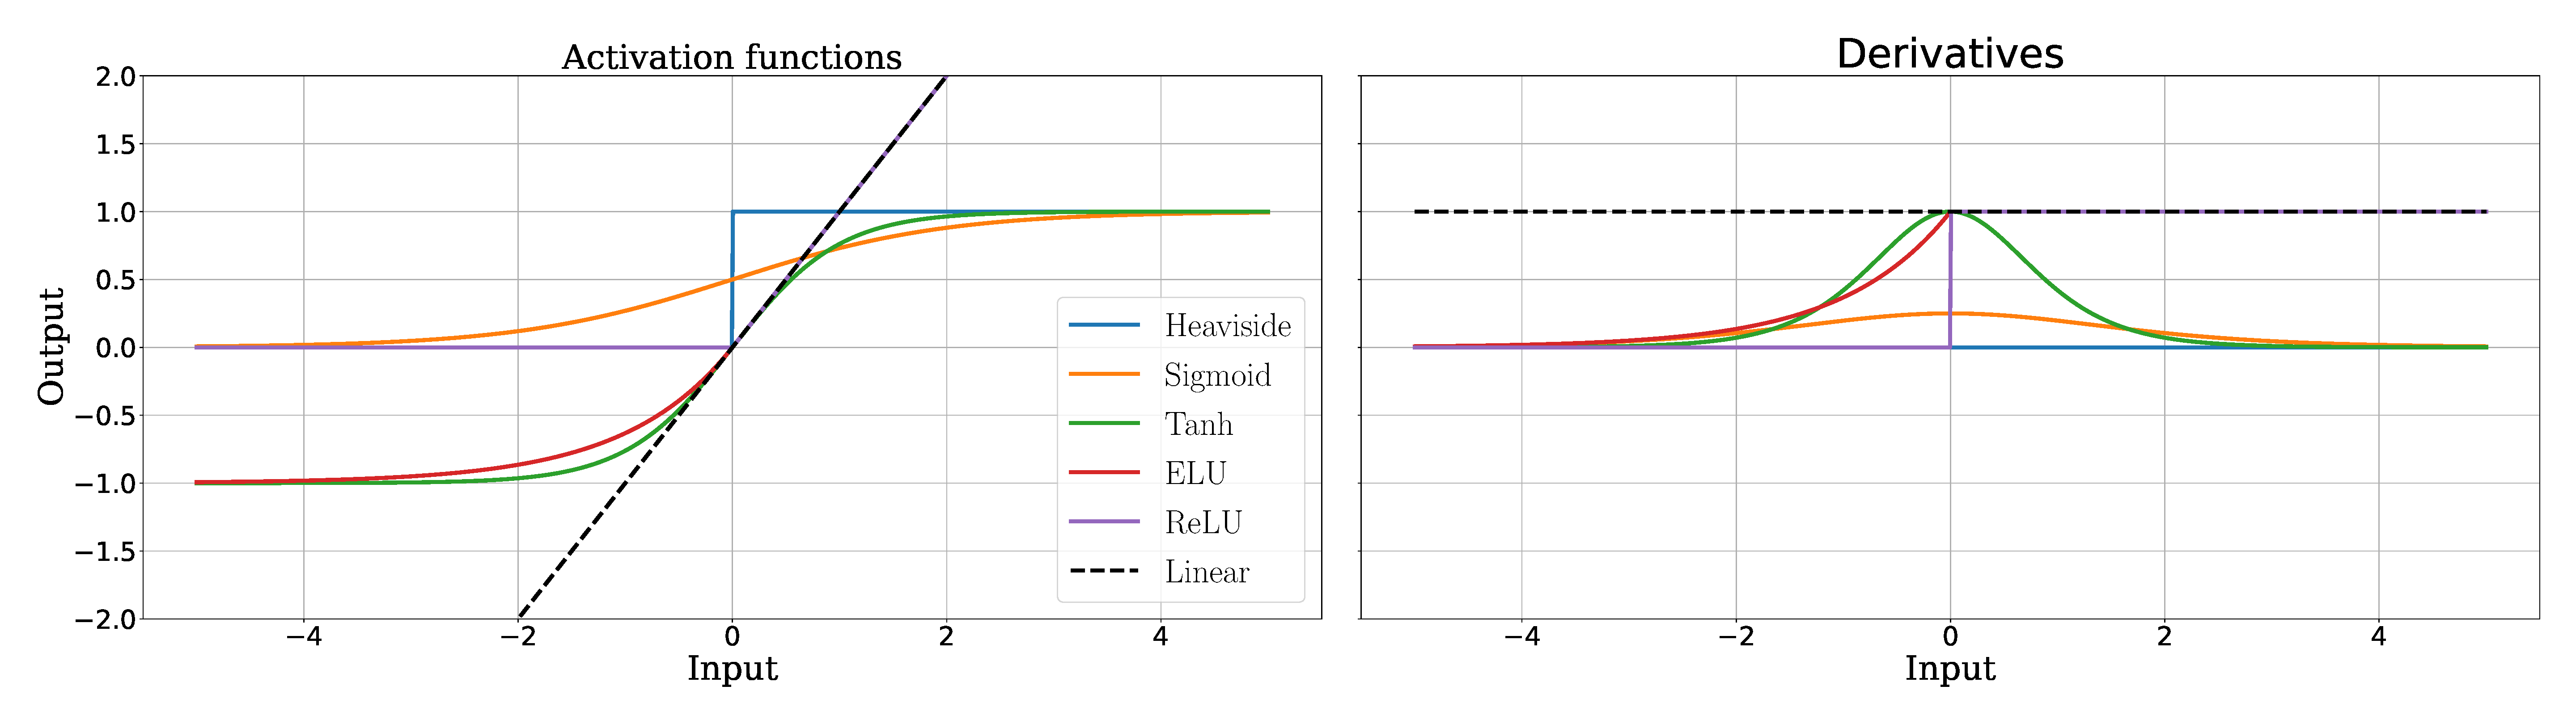
\includegraphics[width=0.98\textwidth]{chapters/foundations/sections/ml/images/activations.pdf}
	\caption[Activation functions]{A selection of different commonly used activation functions on the left and their derivatives on the right.}\label{fig:activations}
\end{figure}

With this, today's definition of a neuron is given by
\begin{equation}\label{eq:def-neuron}
n: \R^m\times \R^m\times \R \to \R;\ \lr{\vec{x}, \vec{w}, b}\mapsto a\lr{\vec{w}\cdot\vec{x} + b}.
\end{equation}
A diagram of a modern neuron is shown in \autoref{fig:neuron}. In general a \acrshort{nn} consists of arbitrary connections of these kinds of neurons, that allow for the representation of more complex functions.

\begin{figure}
	\centering
	\begin{tikzpicture}
\node[draw, circle, minimum size=0.75cm] (neuron) {};
\node (z) [below=0.1cm of neuron] {$z = \vec{w}\cdot\vec{x}+b$};
\node (x_1) [left=1.5cm of neuron] {$x_1$};
\node (x_0) [above=0.5cm of x_1] {$x_0$};
\node (x_2) [below=0.5cm of x_1] {$x_2$};
\node (a) [right=1.5cm of neuron] {$a\lr{z}$};

\draw[->, shorten >= 2pt] (x_0) -- (neuron) node[midway, above] {$w_0$};
\draw[->, shorten >= 2pt] (x_1) -- (neuron) node[midway, above] {$w_1$};
\draw[->, shorten >= 2pt] (x_2) -- (neuron) node[midway, above] {$w_2$};

\draw[->, shorten >= 2pt] (neuron) -- (a);
\end{tikzpicture}
	\caption[Single artificial neuron]{Depiction of a single neuron. It takes a three dimensional input $\vec{x}=\lr{x_0, x_1, x_2}^T$ and has four parameters; the weights $\vec{w}=\lr{w_0, w_1, w_2}^T$ and the bias $b$. Its output is the activation $a$ applied to $z=\vec{w}\cdot \vec{x}+b$.}\label{fig:neuron}
\end{figure}

However, when defining a \acrshort{nn} it is often convenient to take a more structured approach. The individual neurons can be combined into layers. Each neuron in the layer is then required to have the same inputs and the same activation function. As such a layer of neurons is a function
\begin{equation}\label{eq:def-layer}
\mathcal{L}: \R^m\times\R^{l\times m}\times\R^l\to\R^l;\ \lr{\vec{x}, W, \vec{b}}\mapsto a\lr{W\cdot \vec{x} + \vec{b}},
\end{equation}
where $W$ is the weight-matrix, consisting of the weights of each neuron stacked in the rows, and $\vec{b}$ summarizing the biases of the different neurons. The activation function $a$ is understood to operate component-wise on its argument.

To form a \acrshort{nn}, these layers can then be connected. In its most simple form, a \acrshort{nn} is a set of nested layers:
\begin{equation}\label{eq:def-fnn}
\mathcal{N}\lr{\vec{x}, \theta} = \mathcal{L}_n\lr{\mathcal{L}_{n-1}\lr{\dots \mathcal{L}_1\lr{\vec{x}, \theta_1},\dots \theta_{n-1}}, \theta_n}.
\end{equation}
The values $\theta_i = \lr{W_i, \vec{b}_i}$ are collectively called the parameters of the layer and $\theta=\lr{\theta_1, \dotsc, \theta_n}$ are the parameters of the network.

Equation \eqref{eq:def-fnn} defines a \emph{feed forward neural network}. Information flows only in one direction, from the input $x$, through the intermediate layers $\mathcal{L}_1, \mathcal{L}_2, \cdots, \mathcal{L}_{n-1}$, to the output $\mathcal{L}_n$. No feedback connections are allowed and the resulting graph is acyclic~\cite{Goodfellow:2016:DNN}. When the graph does contain cycles, the resulting network is known as a \emph{recurrent neural network} (\acrshort{rnn})~\cite{Rumelhart:1986aaa, Elman:1990aaa}. These have traditionally had many applications in different kinds of natural language processing (\acrshort{nlp})~\cite{Yin:2017aaa} and are viewed as resembling biological brains more closely. They were even considered as a central idea in the original works by McCulloch and Pitts~\cite{McCulloch:1943, Piccinini:2004}. However, feed forward \acrshort{nn}s tend to be easier to optimize than \acrshort{rnn}s and variants of feed forward \acrshort{nn}s have started to perform better than state-of-the-art \acrshort{rnn}s~\cite{Vaswani:2017aaa, Tunstall:2022aaa}. For these reasons my works have exclusively considered feed forward \acrshort{nn}s. I point the interested reader to chapter 10 of~\cite{Goodfellow:2016:DNN} and chapters 15 and 16 of~\cite{Geron:2017aaa} for more detail. When talking about \acrshort{nn}s from here on out I will exclusively refer to feed forward \acrshort{nn}s unless otherwise stated.

A \acrshort{nn} can generally be structured into three parts, as illustrated in \autoref{fig:neural_net}. The first part is the \emph{input layer} that passes its inputs unchanged. It has not been stated explicitly in the discussion above and is represented by the input vector $\vec{x}$ in equation \eqref{eq:def-fnn}. Its shape is, therefore, dictated by the example data. The final layer $\mathcal{L}_n$ is the \emph{output layer} and its shape is determined by the desired output of the network. All intermediate layers $\mathcal{L}_1$ to $\mathcal{L}_{n-1}$ in equation \eqref{eq:def-fnn} are called \emph{hidden layers}. The name stems from the fact that the use of these layers is not dictated by the data but fully determined by the learning algorithm~\cite{Goodfellow:2016:DNN}. The state is basically hidden to the outside observer, i.e. one can generally not determine the structure of the \acrshort{nn} just from considering outputs on example data. 

\begin{figure}
	\centering
	\begin{tikzpicture}[
	neuron/.style={draw, circle, minimum size=1cm},
	inp/.style={fill=blue, fill opacity=0.4, draw=blue, draw opacity=0.7},
	hid/.style={fill=Emerald, fill opacity=0.4, draw=Emerald, draw opacity=0.7},
	ops/.style={fill=red, fill opacity=0.4, draw=red, draw opacity=0.7},
	conn/.style={->, shorten >= 4pt}
]
% Input layer
\node[neuron, inp] (i0) {};
\node[neuron, inp] (i1) [below=0.5cm of i0] {};
\node[neuron, inp] (i2) [below=0.5cm of i1] {};

% Hidden layers
\node[neuron, hid] (h3) [right=1.5cm of i1] {};
\node[neuron, hid] (h2) [above=0.5cm of h3] {};
\node[neuron, hid] (h1) [above=0.5cm of h2] {};
\node[neuron, hid] (h4) [below=0.5cm of h3] {};
\node[neuron, hid] (h5) [below=0.5cm of h4] {};

\node[neuron, hid] (h12) [right=1.5cm of h1] {};
\node[neuron, hid] (h22) [right=1.5cm of h2] {};
\node[neuron, hid] (h32) [right=1.5cm of h3] {};
\node[neuron, hid] (h42) [right=1.5cm of h4] {};
\node[neuron, hid] (h52) [right=1.5cm of h5] {};

% Output layer
\node[neuron, ops] (o1) [right=1.5cm of h32] {};

%Labels
\node (x0) [left=1cm of i0] {$x_1$};
\node (x1) [left=1cm of i1] {$x_2$};
\node (x2) [left=1cm of i2] {$x_3$};

\node (out1) [right=1cm of o1] {$o_1$};

\node (helper1) [above=0.5cm of h1] {};

\node (inplay) at (i0 |- helper1) {Input layer};
\node (outlay) at (o1 |- helper1) {Output layer};
\path (inplay) -- (outlay) node[midway] (hidlay) {Hidden layers};


% Connections
% Input to hidden layer 1
\draw[conn] (i0) -- (h1);
\draw[conn] (i0) -- (h2);
\draw[conn] (i0) -- (h3);
\draw[conn] (i0) -- (h4);
\draw[conn] (i0) -- (h5);

\draw[conn] (i1) -- (h1);
\draw[conn] (i1) -- (h2);
\draw[conn] (i1) -- (h3);
\draw[conn] (i1) -- (h4);
\draw[conn] (i1) -- (h5);

\draw[conn] (i2) -- (h1);
\draw[conn] (i2) -- (h2);
\draw[conn] (i2) -- (h3);
\draw[conn] (i2) -- (h4);
\draw[conn] (i2) -- (h5);

% Hidden layer 1 to hidden layer 2
\draw[conn] (h1) -- (h12);
\draw[conn] (h1) -- (h22);
\draw[conn] (h1) -- (h32);
\draw[conn] (h1) -- (h42);
\draw[conn] (h1) -- (h52);

\draw[conn] (h2) -- (h12);
\draw[conn] (h2) -- (h22);
\draw[conn] (h2) -- (h32);
\draw[conn] (h2) -- (h42);
\draw[conn] (h2) -- (h52);

\draw[conn] (h3) -- (h12);
\draw[conn] (h3) -- (h22);
\draw[conn] (h3) -- (h32);
\draw[conn] (h3) -- (h42);
\draw[conn] (h3) -- (h52);

\draw[conn] (h4) -- (h12);
\draw[conn] (h4) -- (h22);
\draw[conn] (h4) -- (h32);
\draw[conn] (h4) -- (h42);
\draw[conn] (h4) -- (h52);

\draw[conn] (h5) -- (h12);
\draw[conn] (h5) -- (h22);
\draw[conn] (h5) -- (h32);
\draw[conn] (h5) -- (h42);
\draw[conn] (h5) -- (h52);

% Hidden 2 to output
\draw[conn] (h12) -- (o1);
\draw[conn] (h22) -- (o1);
\draw[conn] (h32) -- (o1);
\draw[conn] (h42) -- (o1);
\draw[conn] (h52) -- (o1);

% Labels to input
\draw[conn] (x0) -- (i0);
\draw[conn] (x1) -- (i1);
\draw[conn] (x2) -- (i2);

% Output to label
\draw[conn] (o1) -- (out1);
\end{tikzpicture}
	\caption[Neural network]{A  fully connected \acrshort{nn} with two hidden layers of equal size (green). It has an input layer with three neurons (blue) that accepts the input-vector $\vec{x}=\lr{x_1, x_2, x_3}^T$. Its output layer has a single neuron (red) and outputs $o_1$.}\label{fig:neural_net}
\end{figure}

The statement that the design of the hidden layers cannot be obtained from example evaluations of the network follows directly from the \emph{universal approximation theorem}. The theorem states that a feed forward \acrshort{nn} with a linear output layer and at least one hidden layer of sufficient size with a non-linear activation function\footnote{The activation function has to also be \enquote{squashing}. The common sigmoid activation for example fulfills all required conditions for the universal approximation theorem~\cite{Goodfellow:2016:DNN}.} can approximate any finite dimensional Borel measurable function to arbitrary precision~\cite{Goodfellow:2016:DNN, Hornik:1989aaa, Hornik:1990aaa}. In practical terms this means that one can always find a \acrshort{nn} $\mathcal{N}\lr{\vec{x},\theta}$ with appropriate parameters $\theta$ that can approximate a function $f\lr{\vec{x}}$. Since only a single hidden layer is required, this also means that any \acrshort{nn} $\widehat{\mathcal{N}}(\vec{x},\hat{\theta})$ can be approximated by a \acrshort{nn} $\mathcal{N}\lr{\vec{x},\theta}$ with just a single hidden layer.

One caveat of the universal approximation theorem is the size of the hidden layer. It is generally not possible to know how large it has to be to approximate any function and greater depth usually leads to better performance. Furthermore, while it is true that effectively most functions can be approximated by some \acrshort{nn}, there is no \acrshort{nn} that is the best for all tasks. This statement can be made even sharper: All \acrshort{ml} algorithms perform equally well when their performance over all possible data generating distributions is averaged~\cite{Goodfellow:2016:DNN}. %page 113
It is known as the \emph{no free lunch theorem} and was proven by Wolpert in 1996~\cite{Wolpert:1996aaa}. However, it does not state that a particular algorithm cannot outperform others for any particular task. It simply means that it is impossible to design an algorithm that is optimal for all tasks.

To conclude this subsection I want to point out that equations \eqref{eq:def-neuron}, \eqref{eq:def-layer}, and \eqref{eq:def-fnn} have only considered vector-valued inputs and functions. This is not required but simplifies notation. In \autoref{sec:cnn} layers with different inputs and outputs will be introduced.


\subsection{Training Neural Networks}\label{sec:nn-training}
The task of training a \acrshort{nn} $\mathcal{N}$ is to use example data in order to find a set of parameters $\theta$ such that $\mathcal{N}\lr{\cdot,\theta}$ suitably approximates a target function $f$. This simple statement already entails the three critical components that are required for training. First we need data sampled from the input domain of $f$. If the algorithm is supposed to be trained in a supervised manner, the corresponding outputs $f\lr{\vec{x}}$ are also required. Second, we need to quantify what it means for $\mathcal{N}$ to be a good approximation to $f$, i.e. we require a performance measure or error-function. Finally, we require a procedure to find parameters $\theta$ that minimize the error between $\mathcal{N}$ and $f$~\cite{Goodfellow:2016:DNN}. %page 149
This subsection will discuss these three aspects and will also touch on a few pitfalls that one may encounter.

The data used to train the \acrshort{nn} is called the \emph{training set}. It is a collection of discrete examples which are used to optimize the parameters $\theta$. As my work has focused solely on supervised learning tasks, for the remainder of this section I will assume that these examples contain both the input as well as the label. While a lot of what is said in this section remains true also for unsupervised learning algorithms, I refer the reader to \cite{Goodfellow:2016:DNN} for more detail.

While the training set is used to optimize the parameters of the \acrshort{nn}, we are only indirectly interested in its performance on this set. If we cared only about the predictions of the network on the training set we could simply create a lookup-table of the examples and would obtain optimal performance. Instead of remembering only the training set, we want the \acrshort{nn} to learn the underlying function $f$. To measure how good this approximation is, we have to measure the performance of the \acrshort{nn} on a second set that is sampled independently from the training set. This second set is called the \emph{test set} and the error obtained on it is known as the \emph{generalization error} or simply \emph{test error}~\cite{Goodfellow:2016:DNN}.

To be able to make statistical statements based on mathematical proofs about the ability to generalize learned features from the training set to the test set, the test set should be sampled not only independently from the training set but also be distributed identically to the training set. Collectively these conditions are called the \emph{i.i.d conditions}. In practice it is most important that the test set is as close to the real application scenario as possible. In my work the training set often consists of discrete samples, while the test set is a continuous time series. This means that both sets are fundamentally not distributed identically. However, both sets are generated with very similar assumptions and thus it is plausible that the \acrshort{nn} will be able to generalize. In fact a core result of our studies is that we are able to optimize our \acrshort{nn}s on the discrete training sets and obtain low, but marginally larger, generalization errors on the continuous test sets.

In order to measure the generalization error a performance measure is required. This performance measure is problem specific but may not always be computationally efficient to calculate or even tractable. Furthermore, for the optimization algorithms that will be discussed below it is vital that the error function is differentiable. Therefore, instead of optimizing the true performance measure one often optimizes a substitute error function instead, in the hope that the two are correlated~\cite{Goodfellow:2016:DNN}. %page 268
This error function in deep learning is known as the \emph{loss} or \emph{cost-function} and the name comes from the fact that it penalizes errors. If instead it rewards good performance, it is called the \emph{fitness function}~\cite{Geron:2017aaa}. %page 20
In deep learning the use of a loss function is more prominent. Mathematically, the loss is a function
\begin{equation}
L: \R^m\times\R^m\to\R;\ \lr{y, \hat{y}}\mapsto L\lr{y, \hat{y}},
\end{equation}
where $y$ is the label and $\hat{y}$ is the predicted output of the network. The lower the loss-values the closer the network is supposed to approximate the function. When the loss is calculated for the entire training or test set it is averaged over all examples.

For certain purposes the loss may also depend directly on other variables, most notably the parameters of the network. We ignore this case here as it is not relevant to my work, but note that including the parameters can force certain behavior of the network. For example, one can push the weights of the network to be numerically small, which can have desirable properties~\cite{Goodfellow:2016:DNN}.

While the loss can in general be freely chosen to suite the task that should be solved, it is often at least partially inspired by a maximum likelihood principle. For instance, if we assume the labels $y$ of the input data $x$ to be drawn from a normal distribution, it is sensible to train the network to estimate the mean of that distribution. Assuming further that the variance $\sigma^2$ of the underlying distribution $y=f\lr{x}$ is fixed, the network that approximates the data generating process best will be the one that maximizes the likelihood
\begin{align}\label{eq:mse-derivation}
\sum_{i=1}^M\log\left[p\lr{y_i\given x_i, \theta}\right] & = \sum_{i=1}^M\log\left[N\lr{y_i, \hat{y}_i, \sigma^2}\right]\nonumber\\
& = -M\log\left[\sigma\right] - \frac{M}{2}\log\left[2\pi\right] - \frac{1}{2\sigma^2}\sum_{i=1}^M{\left|\left|\hat{y}_i - y_i\right|\right|}^2,
\end{align}
where $\hat{y}_i = \mathcal{N}\lr{x_i, \theta}$, $N\lr{y_i, \hat{y}_i, \sigma^2}$ is the normal distribution with mean $\hat{y}_i$ and variance $\sigma^2$ evaluated at the point $y_i$, and $\lr{x_i, y_i}$ are the examples from the training set. Maximizing equation \eqref{eq:mse-derivation} by tuning only the parameters $\theta$ is equivalent to minimizing
\begin{equation}
\text{MSE} = \frac{1}{M}\sum_{i=1}^M {\left|\left|\hat{y}_i - y_i\right|\right|}^2,
\end{equation}
which is known as the \emph{mean squared error} (\acrshort{mse})~\cite{Goodfellow:2016:DNN}. %page 130
This function is commonly used as a loss in regression tasks and I have utilized it in many of my works.

Another common task in machine learning is binary classification. Defining a loss function inspired by a maximum likelihood principle in that case is not trivial, as the conditional probability, too, is binary and as such is not continuous. In this case one often uses a sigmoid activation function (see equation \eqref{eq:def-sigmoid}) on the output layer of the network and interprets the output as a probability. In this case the negative log-likelihood divided by $M$ is given by~\cite{Goodfellow:2016:DNN}%page 137
\begin{equation}
\text{Binary Cross-Entropy} = - \frac{1}{M} \sum_{i=1}^M \lr{y_i\log\left[\hat{y}_i\right]+\lr{1 - y_i}\log\left[1 - \hat{y}_i\right]},
\end{equation}
which is known as the \emph{cross-entropy loss} function or \emph{binary cross-entropy loss} function~\cite{Geron:2017aaa}. %page 149
In case the output layer has $n$ neurons and the labels are one-hot encoded, the loss can be generalized to the \emph{categorical cross-entropy}
\begin{equation}
\text{Categorical Cross-Entropy} = - \frac{1}{M} \sum_{i=1}^M \sum_{j=1}^n y_{i, j}\log\left[\hat{y}_{i, j}\right].
\end{equation}
A one-hot encoded vector has a single entry with the value of $1$, whereas the remaining entries are $0$. Alongside the \acrshort{mse}, the categorical cross-entropy was the most used loss function in my works.

The third component required to train a \acrshort{nn} is an \emph{optimizer} that adjusts the parameters $\theta$. The goal of the optimizer is to minimize the loss on the training set. \acrshort{nn}s as introduced in \autoref{sec:nn} are generally highly complex, non-linear functions that require non-convex optimization. Therefore, it is usually not possible to analytically find the optimal parameters for the network. However, if we consider a fixed example or set of examples from the training set, the loss indirectly becomes a function that depends only on the parameters of the network $\theta$. Minima of that function are extremal points and have a vanishing gradient. Furthermore, the gradient points in the direction of larger values and so one lowers the loss by taking a sufficiently small step in the opposite direction of the gradient (see \autoref{fig:gradient}). This concept is known as \emph{gradient descent} and its usage requires the existence of a derivative of the loss function~\cite{Goodfellow:2016:DNN}. % page 80
With
\begin{equation}\label{eq:total-loss}
J\lr{\theta}=\frac{1}{M}\sum_{i=1}^M L\lr{y_i, \hat{y}_i=\mathcal{N}\lr{x_i, \theta}}
\end{equation}
the parameters of the network are updated as~\cite{Goodfellow:2016:DNN}% page 
\begin{equation}\label{eq:gradient-update}
\theta\to\theta-\eta\nabla_\theta J\lr{\theta},
\end{equation}
where $\eta$ is the learning rate that controls how far the parameters are moved along the error surface of the loss function in the opposite direction of the gradient. Small values of $\eta$ lead to very accurate optimization but potentially require many steps to reach an optimal value. Large values on the other hand lead to quick improvements but risks overshooting minima~\cite{Goodfellow:2016:DNN}. %page 287
Therefore, the learning rate usually has to be adjusted by trial and error to be as large as possible while still reaching low values of the loss.

\begin{figure}
	\centering
	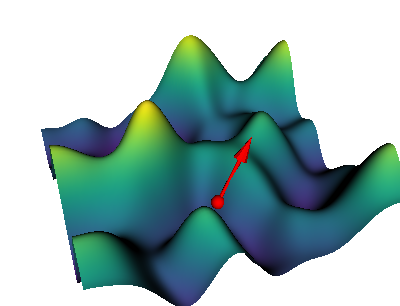
\includegraphics[width=0.6\textwidth]{chapters/foundations/sections/ml/images/gradient.png}
	\caption[Gradient]{Visualization of the gradient of a cost function for a two dimensional parameter space. The height on the vertical axis and the color represent the value of the cost function. The gradient is evaluated at the location of the red dot and is represented by the red arrow. It points in the direction of the largest positive incline. Moving a small step in the oposite direction will reduce the value of the cost function, which is the idea behind gradient descent.}\label{fig:gradient}
\end{figure}

The gradient in equation \eqref{eq:gradient-update} is calculated on the entire training set. To take multiple steps, the calculations have to be repeated on the entire training set. One such pass on the training set is called an \emph{epoch}. Since the entire training set has to be used to calculate a single step, gradient descent scales linearly with the size of that set. As it can be shown that the generalization error falls when the size of the training set increases, \acrshort{nn}s are usually trained on very large sets~\cite{Goodfellow:2016:DNN}. %page 111
This can make the use of full gradient descent computationally prohibitive.

A cheaper alternative to gradient descent is \emph{stochastic gradient descent} (\acrshort{sgd}). Instead of using the entire training set, a random subset, known as a \emph{mini-batch}, is selected. The gradient is subsequently approximated using only the examples from the mini-batch. This procedure has multiple advantages. First, it reduces the computational cost of a single update to the network parameters and forces it to be constant with regards to the size of the training set. Updating the network more often with an approximation of the gradient has proven to reduce wall-clock training time significantly~\cite{Goodfellow:2016:DNN}. %page 148/149
Second, the error between the approximate version and the full gradient scales as $1/\sqrt{n}$, where $n$ is the size of the mini-batch~\cite{Goodfellow:2016:DNN}. %page 271
It, therefore, scales slower than the cost of calculating the gradient and one can balance computational efficiency against the quality of the gradient approximation. Third, using a random subset reduces redundant calculations. In the extreme case, where all examples in the training set are the same, calculating the gradient on the entire training set is equivalent to calculating it on a single example. In a realistic case many examples from the training set may have similar effects on the gradient and applying the update to the parameters earlier leads to faster convergence ~\cite{Goodfellow:2016:DNN}. %page 271
Finally, the stochastic nature introduces randomness into the parameter update steps taken. This may be beneficial when the algorithm finds a local minimum of the loss function, which gradient descent would be unable to get out of. However, this randomness also prevents the algorithm to settle into true minima. In practice, this is a minor issue when mini-batch sizes are not too small and the advantages outweigh the drawbacks~\cite{Geron:2017aaa}. %page 124
A more sophisticated version of \acrshort{sgd} known as ``Adam'' will be discussed at the end of this subsection as it was the optimizer I primarily used in my works.

\acrshort{sgd} is not mathematically guaranteed to arrive even at a local minimum, but practical application have shown that it is capable of reaching sufficiently small values in most cases~\cite{Goodfellow:2016:DNN}. %page 150
To improve optimization further, the whole training set can be shuffled and used for another iteration of \acrshort{sgd}. Since the entire training set is reused in this case, one full pass on it is also called an epoch.

While \acrshort{sgd} describes how to change the network parameters once the gradient is known, it does not provide means to obtain it. This step was the major roadblock for deep learning which was resolved with the introduction of the \emph{backpropagation} algorithm, or simply \emph{backprop}, by Rumelhart, Hinton, and Williams in 1986~\cite{rumelhart1985:aaa}. At its core, backprop is a simple application of the chain rule of derivatives. However, it also utilizes the structured nature of the \acrshort{nn}s to save redundant calculations and thus enables an efficient computation of the gradient. Due to its importance to the field of deep learning, I will introduce the algorithm in the following paragraphs in a bit more detail.

The goal of backpropagation is to efficiently calculate $\nabla_\theta J\lr{\theta}$. For simplicity we assume $J$ to be of the form introduced in \eqref{eq:total-loss}, i.e. the loss function depends on the parameters $\theta$ only through the network. In this case we can focus on calculating the gradient of the per-example loss $L\lr{y_i, \hat{y}_i}$. For simplicity we, furthermore, assume that the output of the network $\hat{y}$ is a vector. If it is not, we apply a reshaping operation that orders the outputs to be of vector form. For readability we also drop the example index $i$ and understand that the following calculations are done for a single example. By the chain rule we then find~\cite{Goodfellow:2016:DNN}%page 199 + 205 f.
\begin{equation}\label{eq:backprop-1}
\lr{\nabla_\theta L\lr{y, \hat{y}}}_i = \frac{\partial \hat{y}^j}{\partial\theta_i} \frac{\partial L\lr{y, \hat{y}}}{\partial \hat{y}^j}=\lr{\nabla_\theta \hat{y}\cdot \nabla_{\hat{y}} L\lr{y, \hat{y}}}_i,
\end{equation}
which uses the Einstein summation convention. The rightmost part in equation \eqref{eq:backprop-1} $\nabla_{\hat{y}} L\lr{y, \hat{y}}$ is the gradient of the loss function with respect to the network output. This can be calculated analytically once and is then evaluated for each example simply by inserting the corresponding network output. The other part is the Jacobian of the network with respect to its parameters
\begin{equation}
\nabla_\theta \hat{y} = \nabla_\theta \mathcal{N}\lr{x, \theta}.
\end{equation}
We assume the network to be a simple chain of layers as defined in \eqref{eq:def-layer}. Once the backpropagation algorithm has been developed for this case, extending it to branching networks is trivial. For easier notation it is helpful to define the recursive relation $z_i\coloneqq W_i a_{i-1}\lr{z_{i-1}}+\vec{b}_i$, with the stopping condition $z_0 = x$ and $a_0$ being the identity mapping. Let $\nabla_{\theta_i}\hat{y}$ be the gradient of $\hat{y}$ only with respect to the parameters of layer $i$. With this we find
\begin{align}\label{eq:backprop_recursive}
\nabla_{\theta_i} \mathcal{N}\lr{x, \theta} = \nabla_{\theta_i}a_n\lr{z_n} & \overset{i < n}{=}\lr{\nabla_{\theta_i}z_n}\cdot\nabla_z a_n\Bigr|_{z=z_n}\nonumber\\
& \overset{\hphantom{i < n}}{=} W_n\nabla_{\theta_i}a_{n-1}\lr{z_{n-1}}\cdot\nabla_z a_n\Bigr|_{z=z_n},
\end{align}
which is a recursive relation for $\nabla_{\theta_i}a_n\lr{z_n}$ that stops on layer $i$. $n$ is the number of layers of the network. Note that while the calculations above suggest that $W_i$ have to be matrices and $z_i$ have to be vectors, the equations hold for tensors of arbitrary dimension. A few things about equation \eqref{eq:backprop_recursive} are noteworthy. First, $a_i$ are scalar functions that are applied component wise. To calculate the gradient $\nabla_z a_i$, the one-dimensional derivative $\partial_z a_i$ simply has to be evaluated at the different values of $z_i$. So the derivative for each activation function $a$ has to be computed analytically in advance only once and can then be used to rapidly calculate the gradients $\nabla_z a_i$. Second, since \eqref{eq:backprop_recursive} is a recursive equation, the gradient at layer $n-i$ depends on all gradients from layer $n-i+1$ to $n$. This is where the name backpropagation comes from, as the gradients are propagated back through the network. The recursion stops on layer $i$
\begin{equation}\label{eq:backprop-rec-stop}
\nabla_{\theta_i} a_i\lr{z_i} = \lr{\nabla_{\theta_i} W_i} a_{i-1}\lr{z_{i-1}}+\nabla_{\theta_i}\vec{b_i}.
\end{equation}

For practical implementations, the backprop algorithm is comprised of two stages. First, the input data is passed through the network and the activations $z_i$ are stored for every layer. This operation is known as the \emph{forward pass}. The second step uses the data from the forward pass to iteratively compute the gradient using equations \eqref{eq:backprop-1}, \eqref{eq:backprop_recursive}, and \eqref{eq:backprop-rec-stop}. This is referred to as the \emph{backward pass}.

In principle the calculation of the gradient could be done sequentially. In real applications this is often impractical, since \acrshort{gpu}s allow for high degrees of parallelization. Therefore, many, if not all, examples from a mini-batch are evaluated at the same time. Since the backprop algorithm requires to store the output of all intermediate layers, the memory requirements during training scale linearly with the mini-batch size. This was a limiting factor for many of our works and usually required us to use small mini-batches. Furthermore, a computational graph is usually built which describes the operations and their order that need to be taken to compute the output of the \acrshort{nn} given its input. Each node in this graph then needs to implement a backprop-method that returns the gradient of that node given any of its inputs and an inbound gradient.

As an example consider the matrix multiplication operation $C=AB$. Its backprop-method needs to return $GB^T$ when it is called for input $A$ and inbound gradient $G$ and $A^TG$ if it is called for input $B$. For a more thorough discussion of how the computational graphs are built I refer the reader to chapter 6 of~\cite{Goodfellow:2016:DNN}, where the above example was taken from.

With the definition of a training and test set, the loss function, and \acrshort{sgd} in combination with backprop we have developed the most important tools to train a \acrshort{nn}. However, during training multiple problems can arise. I will now discuss the most common ones and how to characterize them.

\subsubsection{Common problems during training}
One of the most challenging problems of deep learning is the training setup. How does one choose a network structure that is capable of efficiently solving a given problem? The structure of a \acrshort{nn} is most commonly referred to as the \emph{architecture} of the network and designing it is often more of an art than a science. Certain conditions, like translation invariance of the problem or hardware resource limitations, may inform or constrain it, but most of the time, the architecture is found empirically.

Another part of the training setup is the optimizer. It, too, can greatly influence how efficiently a \acrshort{nn} learns. Even the simple \acrshort{sgd} optimizer discussed above has a free parameter, the learning rate $\eta$. Setting it too large or too small may have detrimental results on the ability of the \acrshort{nn} to learn. More complex optimizers, such as Adam \cite{Kingma:2014aaa}, often have a larger number of tunable parameters and setting them correctly can be challenging. To find good settings for the optimizer, one usually has to resort to trial and error as well.

Both the architecture and the parameters of the optimizer have in common that they are set outside of the training loop. They can, therefore, not be updated automatically. Parameters that control the behavior of the learning algorithm are known as \emph{hyperparameters}~\cite{Goodfellow:2016:DNN}.

To optimize the hyperparameters, one often tests different settings, trains the algorithm, and compares their generalization errors. The settings that yield the best performance are then used. As we are interested in the generalization error, the training set cannot be used for this calculation. On the other hand, using the test set to optimize the hyperparameters would be dangerous, as this would introduce a bias. We would optimize the learning algorithm to perform well on the test set, reducing the ability of said set to measure how well the algorithm can generalize beyond previously observed examples. For this reason a third set is introduced: the \emph{validation set}. With this set, hyperparameters are optimized by choosing specific settings, training the resulting algorithm using the training set, and calculating the error on the validation set. The errors for different hyperparameters are subsequently compared and the model with the best performance is chosen. Finally, the generalization error is calculated on the test set only once on the chosen model to estimate how well the algorithm will perform. The error calculated on the validation set is also called the \emph{validation error}, to differentiate it from the generalization error~\cite{Goodfellow:2016:DNN}.%page 107 ff. + 117 ff.

When a \acrshort{nn} is trained for long periods of time, one can often observe that the network starts to ``remember'' the samples of the training set. To spot this, one can compare the error or loss calculated on the training set to the one calculated on the validation set after every epoch. When the network starts to remember individual samples it stops to generalize and the validation error will grow. This process is known as \emph{overfitting}~\cite{Geron:2017aaa}.%page 27 f.

To understand overfitting, we can consider polynomial regression. Let us imagine that our training set consists of $N$ samples with data $x_i$ and labels $y_i$. Let us further assume that the underlying distribution of our data is the polynomial $p(x)=\sum_{j=0}^M a_j x^j$ of degree $M < N$, i.e. $y_i=\sum_{j=0}^M a_j x_i^j$. If we use a polynomial $\hat{p}(x)=\sum_{j=0}^M \hat{a}_j x^j$ of degree $M$ to fit our training data, we will drive the \acrshort{mse} of the training set to $0$ when $\hat{a}_j = a_j\ \forall j\in\{0, 1, \cdots, M\}$. However, we can also fit all samples from the training set identically when we use a polynomial of any degree $\geq N$~\cite{Goodfellow:2016:DNN}. %page 109f.
Importantly, this fit does not necessarily have to find the coefficients
\begin{equation}
\hat{a}_j =
	\begin{cases}
		a_j,& j \leq M\\
		0,& \text{otherwise}
	\end{cases}
\end{equation}
but may find a different solution. See panels (b) and (c) of \autoref{fig:over_under_fit} for an example. In the case of overfitting the model is too complex for the task that has to be solved~\cite{Goodfellow:2016:DNN}. When the new model of degree $\geq N$ is evaluated on new points, it will most likely make incorrect predictions; it has ``memorized'' the training samples but is incapable of generalizing to new samples.

\begin{figure}
	\centering
	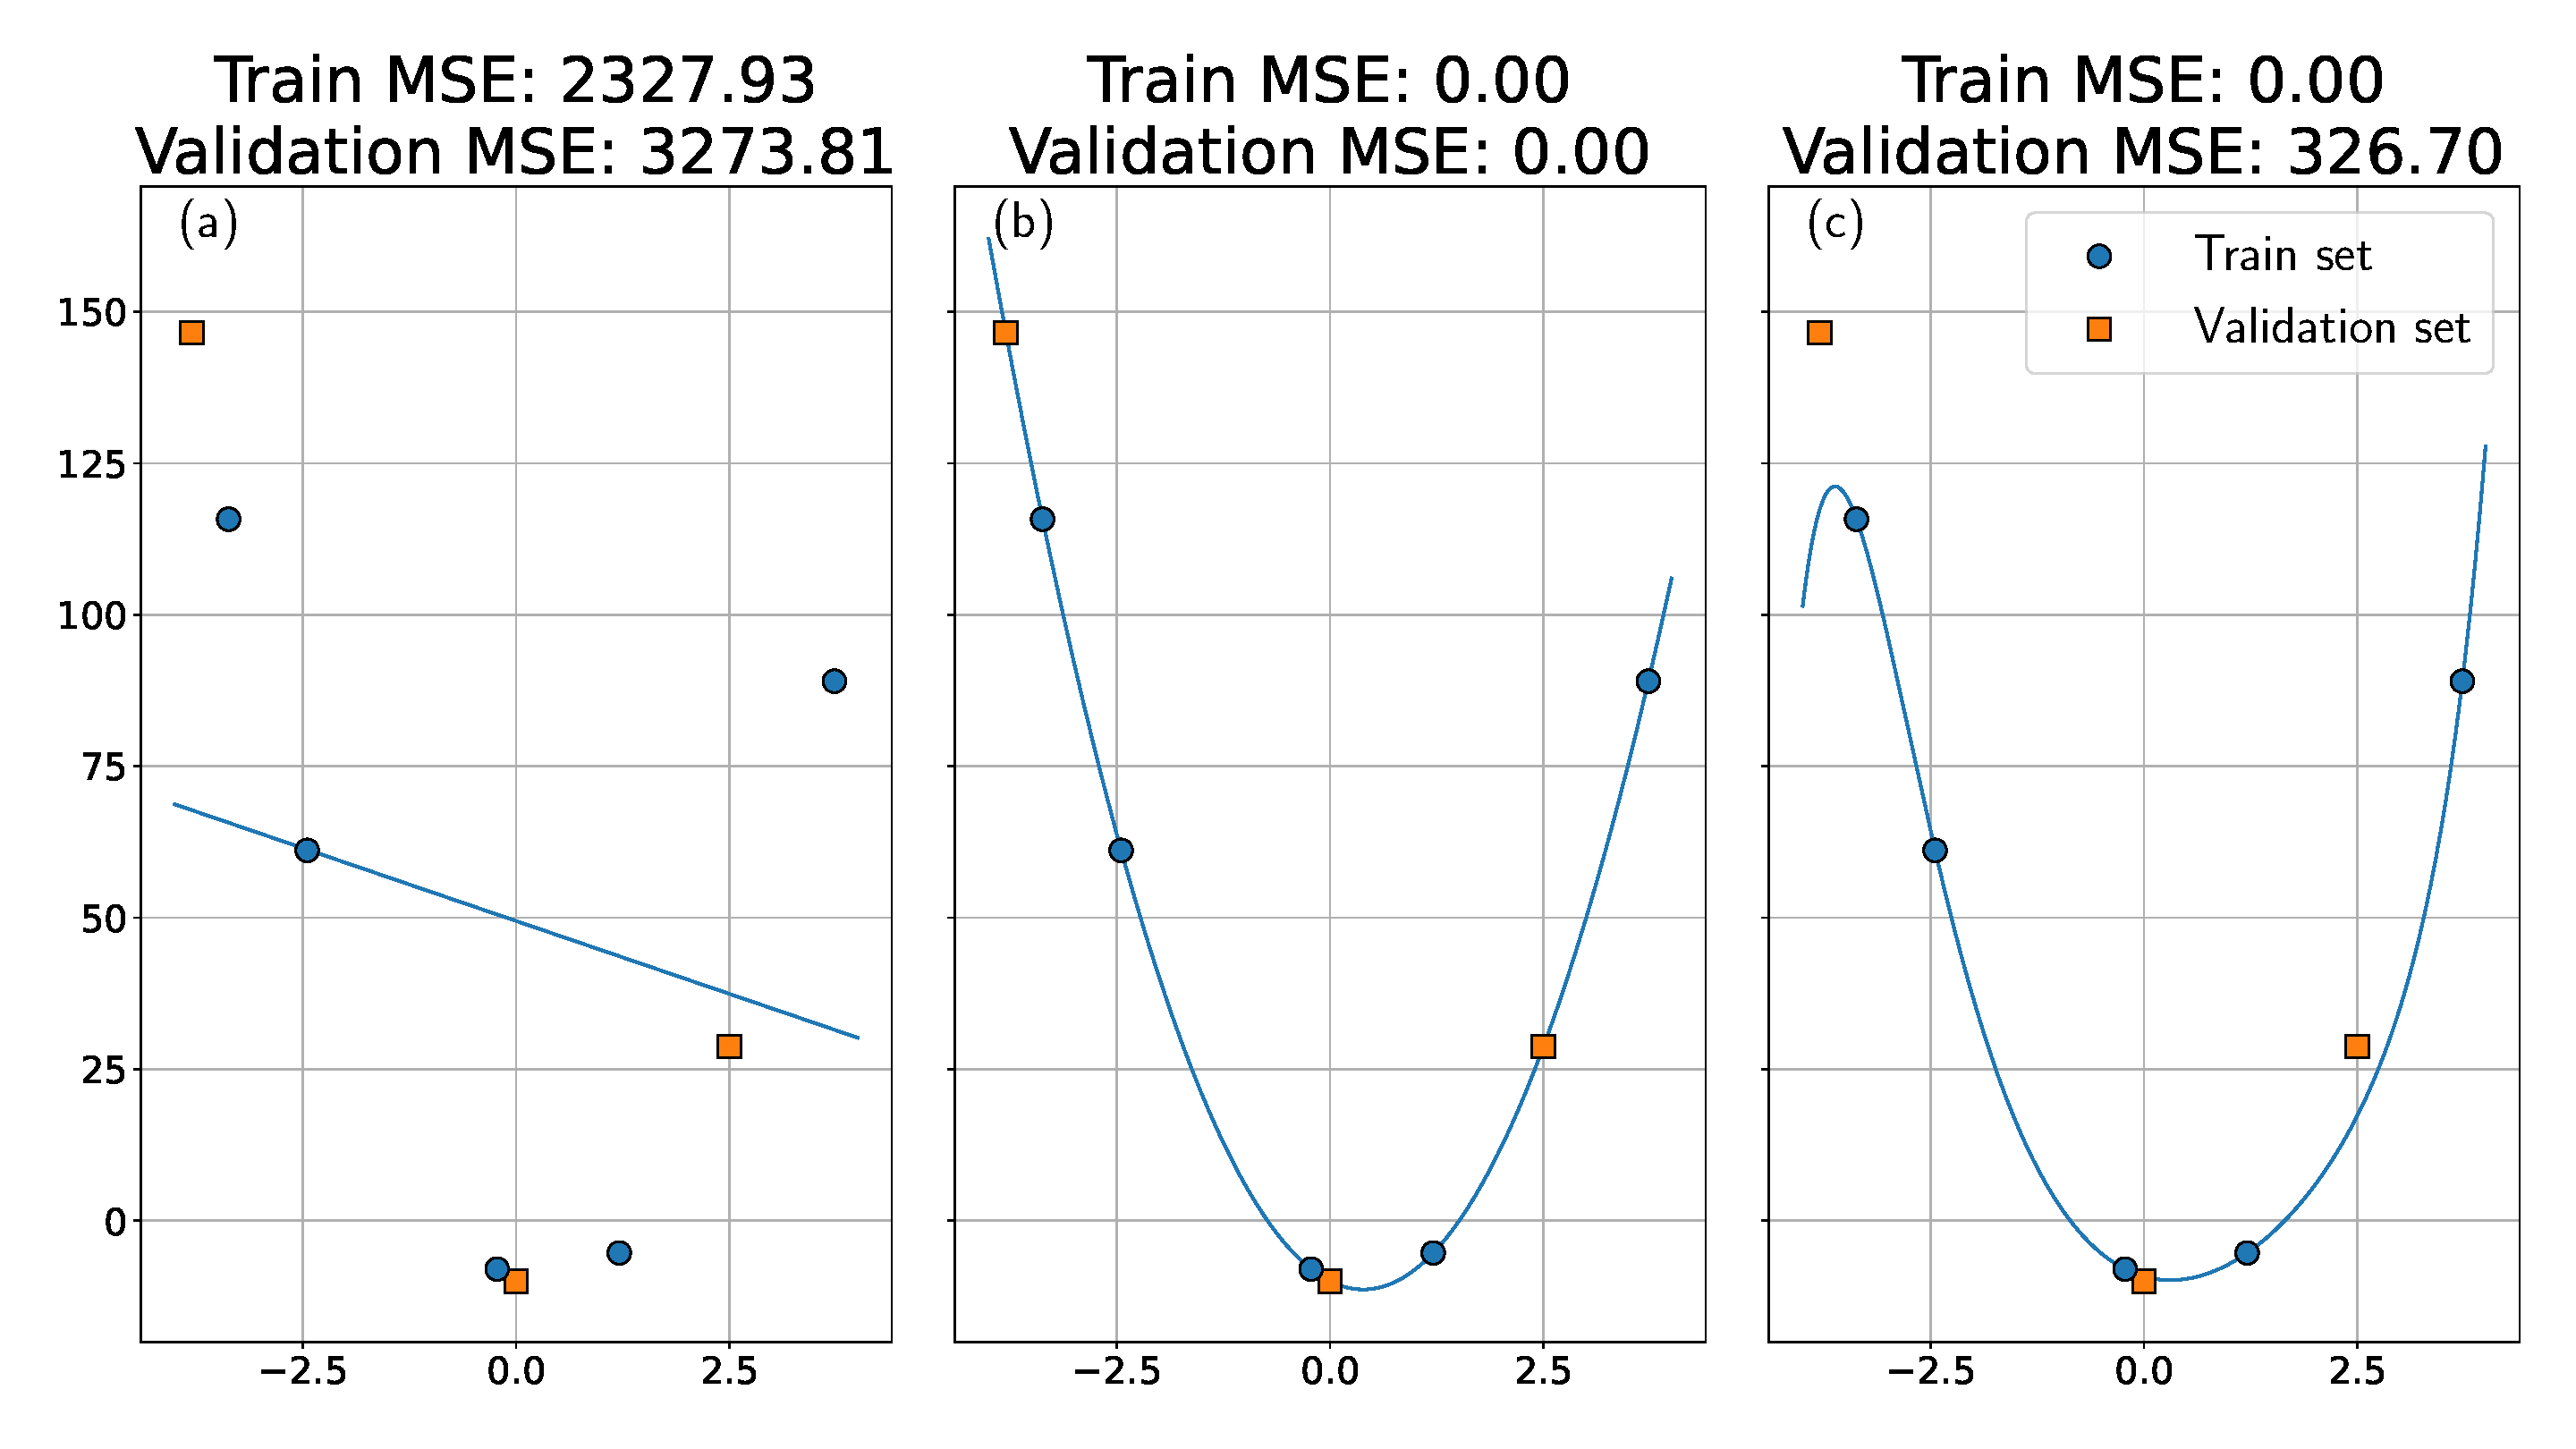
\includegraphics[width=0.98\textwidth]{chapters/foundations/sections/ml/images/overunderfit.pdf}
	\caption[Over- and underfitting]{Polynomials of different degrees fitting the same training data using a least squares fit. The training data is generated from the second degree polynomial shown in panel (b). All panels list the \acrshort{mse} of the fit against the training and validation data on top. In panel (a) a linear model is used to fit the data. It is not complex enough and underfits the data. Panel (b) is a second degree polynomial that optimally fits the data. It minimizes the \acrshort{mse} on both the training and validation set. Panel (c) fits a 9th degree polynomial to the training set. It overfits and cannot generalize well to the unseen validation data. This figure was inspired by figure 5.2 of \cite{Goodfellow:2016:DNN}.}\label{fig:over_under_fit}
\end{figure}

There are two options to reduce overfitting. One can either decrease the model complexity or increase the number of samples in the training set. As data could be generated at little additional cost for most of the studies in this work, we have usually chosen to take the latter approach~\cite{Goodfellow:2016:DNN, Geron:2017aaa}.

Instead of the model being too complex for the problem, the opposite may also happen. When the model is inherently not capable of representing the underlying data distribution, it is \emph{underfitting} the data. In the example of polynomial regression above, any polynomial of degree $<M$ would most likely be incapable of matching the training data. Panel (a) of \autoref{fig:over_under_fit} shows an example~\cite{Goodfellow:2016:DNN}.

Spotting underfitting is often a lot more challenging than spotting overfitting, because it keeps the error calculated on the training set large. However, the same effect happens, when the network has not yet converged to a good local minimum of the loss. Furthermore, one rarely knows a priory what a good value for the converged loss would be. Upper limits can often be derived, but those usually cover the network not being able to optimize at all, rather than it failing to suitably approximate the true data distribution. Once underfitting has been identified though, one can usually increase the number of trainable parameters of the \acrshort{nn} to resolve the issue. Other times finding a more suitable architecture or different data representation is required.

Another common problem of deep neural networks are vanishing or exploding gradients~\cite{Goodfellow:2016:DNN,Geron:2017aaa,He:2015aaa}. Deeper layers tend to have smaller gradients, which causes a stagnation in their optimization~\cite{Geron:2017aaa}. %page 332
To a certain degree studies have found that the main cause of vanishing gradients were the combination of the network initialization, i.e. the initial parameters of the network, and the activation functions~\cite{Glorot:2010aaa}. But even with improved network initialization and suitable activation functions, training can become difficult beyond a certain depth~\cite{He:2015aaa}.
The opposite can also happen, where gradients grow exponentially. However, this is mostly a problem in \acrshort{rnn}s and can be combated by clipping the norm of the update step~\cite{Goodfellow:2016:DNN}. %page 282


Further failure modes for the training of deep \acrshort{nn}s are discussed in chapter 8.2 of \cite{Goodfellow:2016:DNN}.


\subsubsection{The Adam Optimizer}
All of the works centered around deep learning that are discussed in this thesis make use of the Adam optimizer. For this reason, it is introduced here. Adam stands for ``adaptive moment'' estimation and it computes individual adaptive learning rates for different parameters from estimates of the first and second moments of the gradients~\cite{Kingma:2014aaa}. It can be seen as a variant to the RMSProp algorithm~\cite{Goodfellow:2016:DNN,Tieleman:2012aaa}, which extends the AdaGrad algorithm~\cite{Duchi:2011aaa}.

The core idea of AdaGrad is to scale the learning rate of individual parameters based on the scale of the gradient. In regions where the loss surface is shallow one wants to traverse it fast to reach more optimal values. In regions where the surface has a steep gradient, smaller steps should be taken to not overshoot a potential minimum. To do this, the algorithm aggregates the squared gradients. On each \acrshort{sgd} step the current gradient is then divided by the square root of the aggregated squared gradients.

RMSProp uses an exponential moving average to aggregate the squared gradients. This reduces the memory of gradients from the extreme past and helps to keep the learning rates large enough to converge quickly once a locally convex bowl has been found~\cite{Goodfellow:2016:DNN}. %page 300

Adam uses two exponential moving averages. Instead of just keeping track of the squared gradient, i.e. the second moment of the gradient, it also keeps track of the first moment of the gradient, i.e. its mean. Additionally, it removes biases from the moments. The full algorithm is given in algorithm 1 of \cite{Kingma:2014aaa}. The core calculations of the algorithm in the language used in this thesis are~\cite{Geron:2017aaa}%page 356; happens to use the same notation as me
\begin{align}
1.\ & m \leftarrow \beta_1 m - \lr{1 - \beta_1}\nabla_\theta J\lr{\theta}\nonumber\\
2.\ & s \leftarrow \beta_2 s + \lr{1 - \beta_2}\nabla_\theta J\lr{\theta}\odot\nabla_\theta J\lr{\theta}\nonumber\\
3.\ & \hat{m} \leftarrow \frac{m}{1 - \beta_1^t}\nonumber\\
4.\ & \hat{s} \leftarrow \frac{s}{1 - \beta_2^t}\nonumber\\
5.\ & \theta \leftarrow \theta + \eta\hat{m}\oslash \sqrt{\hat{s}+\epsilon},
\end{align}
where $\beta_1$, $\beta_2$, and $\epsilon$ are hyperparameters of the algorithm, $t$ counts the iterations, and $\odot$ and $\oslash$ are element wise multiplication and division operators, respectively. The default values suggested in \cite{Kingma:2014aaa} are $\beta_1 = 0.9$, $\beta_2 = 0.999$, $\epsilon = 10^-8$, and $\eta = 0.001$.

Steps $1$ and $2$ are the exponential moving averages of the first and second moment of the gradient, respectively. The values for $m$ and $s$ are both initialized as arrays filled with zeros. This initialization would introduce a bias, which is removed by the operations in steps $3$ and $4$. Finally, step $5$ applies the gradient update, which scales the learning rate by the inverse square root of the second moment of the gradients. The gradient updates are also only propagated using the running mean of step $3$.


\subsection{Convolutional Neural Networks}\label{sec:cnn}
The layers discussed in section \ref{sec:nn} connect every input to every neuron. They are known as fully connected or dense layers. A fully connected layer with $N$ inputs and $M$ outputs has a weight matrix of dimension $M\times N$. For large inputs and outputs this can quickly become very straining on both memory and compute power. Furthermore, both the input- and output-shape of the layers must be set at the beginning and cannot change.

All of these problems are being addressed by the convolutional layer which was invented in 1989~\cite{LeCun:1989aaa}. Instead of connecting all inputs to all outputs, it connects only parts of the input to each output neuron. Furthermore, the weights are shared between different connections. In mathematical terms, the layer performs a discrete convolution of a kernel with the input data; hence the name ``convolutional layer''. For 1 dimensional data $\vec{x}$, weights $\vec{w}$, and bias $b$ the layer can be written as
\begin{equation}\label{eq:1dconv_simple}
\mathcal{L}_\text{conv}\lr{x, \theta}_i = a\lr{\sum_j x_j \hat{w}_{i-j} + b},
\end{equation}
where
\begin{equation}
\hat{w}_i = 
	\begin{cases}
		w_i,& 0 \leq i < \text{dim}\lr{\vec{x}}\\
		0,& \text{otherwise}
	\end{cases}.
\end{equation}
The weights $\vec{w}$ in the above equation are often called \emph{kernel}, and when defining a \acrshort{nn} architecture with convolutional layers one often sets the \emph{kernel size}, i.e. the dimension of the kernel.

Depending on the problem, convolutional layers have several advantages over fully connected layers. First, the introduction of sparse connections. This means that not all outputs are connected to all inputs, which reduces the theoretical computational time from $\mathcal{O}\lr{M\times N}$ to $\mathcal{O}\lr{K\times N}$, where $K=\text{dim}\lr{\vec{w}}$. Second, the introduction of shared weights, which reduces memory requirements, as only $K$ rather than $M\times N$ numbers have to be stored for the weights. Third, the introduction of equivariance to translation. This is a direct consequence from sharing parameters and translating them over the input, as it allows to search for the same learned features in multiple locations of the input data. For instance, if a kernel has been optimized to detect edges in an image, it will be able to detect these edges in all parts of the image. A fully connected layer, on the other hand, would need to learn this filter at every location. While this is in principle possible, and one can reduce the convolutional layer to a special case of a fully connected layer when the input size is known\footnote{The weight vector can be zero padded to have the same dimensionality as the input vector. One then cyclicly changes the position of the weight vector in the zero padding and uses the different resulting vectors as rows for the weight matrix of a fully connected layer. See section 9.4 of \cite{Goodfellow:2016:DNN} or \cite{Schaefer:2019:MSC} for more details.}, it is not quite so simple in real applications. If we want to learn to detect a specific edge in all parts of the image, a fully connected layer needs sufficiently many examples of such edges at every location of the image. A convolutional layer might learn the filter even if the edges are only presented in one specific region of the images from the training set~\cite{Goodfellow:2016:DNN}. %page 321 ff.
Additionally, convolutional layers can process inputs of arbitrary size, as the parameters of the layer do not depend on the input.

A single kernel will learn a single filter. For example, the two dimensional filter in the top branch of \autoref{fig:edge-filter} detects vertical edges. It will, however, not be able to also detect horizontal edges. For this reason, a convolutional layer usually has multiple kernels of the same dimensions. It optimizes them in parallel to learn multiple different filters. The outputs of the convolutions with the different kernels are then stacked. The output of a single kernel convolution is known as a \emph{feature map} and the index dimension of the different feature maps is known as the \emph{channel} dimension. The name feature map originates from the observation that the activation at a certain location is particularly large, when the kernel strongly overlaps with a specific feature in the input data~\cite{Zeiler:2014aaa}. Naming different feature maps different channels, stems from RGB-images, which have three distinct channels; one for red (R), one for green (G), and one for blue (B)~\cite{Goodfellow:2016:DNN}.%page 337

\begin{figure}
	\centering
	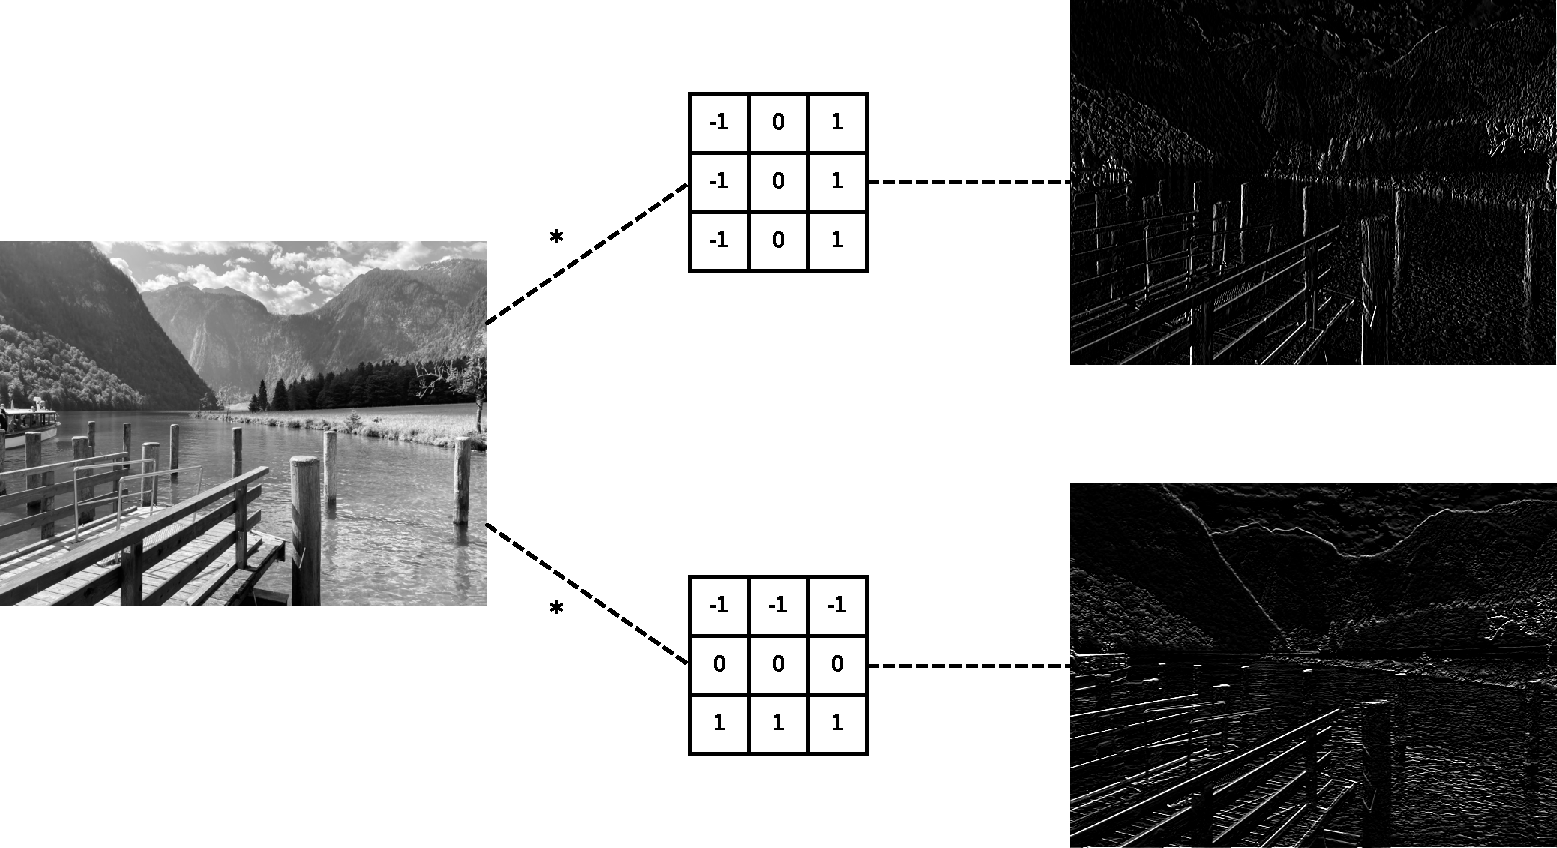
\includegraphics[width=\textwidth]{chapters/foundations/sections/ml/images/edge_filter.pdf}
	\caption[Edge detection convolution]{An image convolved with a vertical (top) and horizontal (bottom) edge-detection kernel. The original image is shown on the left. The processed images are shown on the right. The $\ast$ is the symbol for the convolution operation. Brighter pixels in the output images signify larger values, i.e. a larger overlap between the kernel and the image. On the top branch one can clearly spot the bright vertical edges of the posts, which are not visible in the lower branch. On the other hand, one can clearly spot the sharp edges at the top of the posts in the lower branch but not in the upper branch.}\label{fig:edge-filter}
\end{figure}

As was the case for \acrshort{nn}s consisting only of fully connected layers, greater depth of convolutional neural networks (\acrshort{cnn}s) allow them to detect features of greater complexity. For instance, if the first layer learns one filter for vertical edges and one for horizontal edges, a subsequent layer may use the information from both channels to infer the angle of an edge. For this to be possible, it has to combine the information. Therefore, a single kernel of a one dimensional convolution as defined in equation \eqref{eq:1dconv_simple} spans all channels. If the input to a one dimensional convolutional layer has $n$ samples and $c$ channels, a single kernel $W$ will be of dimension $k\times c$, where $k$ is the kernel size. See \autoref{fig:conv} for a visualization.

\begin{figure}
	\centering
	\begin{subfigure}[b]{.3\linewidth}
		\resizebox{\linewidth}{!}{\begin{tikzpicture}[
neuron/.style={
	regular polygon,regular polygon sides=4, minimum size=2cm, draw
}
]
% Input
\draw[solid, thick] (0, 0) rectangle (1, -1) node[pos=0.5] {$i_{1, 1}$};
\draw[solid, thick] (0, -1) rectangle (1, -2) node[pos=0.5] {$i_{2, 1}$};
\draw[solid, thick] (0, -2) rectangle (1, -3) node[pos=0.5] {$i_{3, 1}$};
\draw[solid, thick] (0, -3) rectangle (1, -4) node[pos=0.5] {$i_{4, 1}$};
\draw[solid, thick] (0, -4) rectangle (1, -5) node[pos=0.5] {$i_{5, 1}$};
\draw[solid, thick] (0, -5) rectangle (1, -6) node[pos=0.5] {$i_{6, 1}$};
\draw[solid, opacity=0] (0, -6) rectangle (1, -7);

\draw[solid, thick] (1, 0) rectangle (2, -1) node[pos=0.5] {$i_{1, 2}$};
\draw[solid, thick] (1, -1) rectangle (2, -2) node[pos=0.5] {$i_{2, 2}$};
\draw[solid, thick] (1, -2) rectangle (2, -3) node[pos=0.5] {$i_{3, 2}$};
\draw[solid, thick] (1, -3) rectangle (2, -4) node[pos=0.5] {$i_{4, 2}$};
\draw[solid, thick] (1, -4) rectangle (2, -5) node[pos=0.5] {$i_{5, 2}$};
\draw[solid, thick] (1, -5) rectangle (2, -6) node[pos=0.5] {$i_{6, 2}$};
\draw[solid, opacity=0] (1, -6) rectangle (2, -7);

% Output
\draw[solid, thick] (6, -0.5) rectangle (7, -1.5) node[pos=0.5] {$o_{1, 1}$};
\draw[solid, thick] (6, -1.5) rectangle (7, -2.5) node[pos=0.5] {$o_{2, 1}$};
\draw[solid, thick] (6, -2.5) rectangle (7, -3.5) node[pos=0.5] {$o_{3, 1}$};
\draw[solid, thick] (6, -3.5) rectangle (7, -4.5) node[pos=0.5] {$o_{4, 1}$};
\draw[solid, thick] (6, -4.5) rectangle (7, -5.5) node[pos=0.5] {$o_{5, 1}$};

\draw[solid, thick] (7, -0.5) rectangle (8, -1.5) node[pos=0.5] {$o_{1, 2}$};
\draw[solid, thick] (7, -1.5) rectangle (8, -2.5) node[pos=0.5] {$o_{2, 2}$};
\draw[solid, thick] (7, -2.5) rectangle (8, -3.5) node[pos=0.5] {$o_{3, 2}$};
\draw[solid, thick] (7, -3.5) rectangle (8, -4.5) node[pos=0.5] {$o_{4, 2}$};
\draw[solid, thick] (7, -4.5) rectangle (8, -5.5) node[pos=0.5] {$o_{5, 2}$};

\begin{scope}[on background layer]
	\draw[fill=red, fill opacity=0.3] (0, 0) rectangle (2, -2);
	\draw[fill=blue, fill opacity=0.3] (0, -3) rectangle (2, -5);
	
	\draw[fill=red, fill opacity=0.3] (6, -0.5) rectangle (7, -1.5);
	\draw[fill=blue, fill opacity=0.3] (7, -3.5) rectangle (8, -4.5);
\end{scope}

\draw[solid, draw=black] (3, 0) rectangle (4, -1) node[pos=0.5] {$w^1_{1,1}$};
\draw[solid, draw=black] (4, 0) rectangle (5, -1) node[pos=0.5] {$w^1_{1,2}$};
\draw[solid, draw=black] (3, -1) rectangle (4, -2) node[pos=0.5] {$w^1_{2,1}$};
\draw[solid, draw=black] (4, -1) rectangle (5, -2) node[pos=0.5] {$w^1_{2,2}$};

\draw[solid, draw=black] (3, -3) rectangle (4, -4) node[pos=0.5] {$w^2_{1,1}$};
\draw[solid, draw=black] (4, -3) rectangle (5, -4) node[pos=0.5] {$w^2_{1,2}$};
\draw[solid, draw=black] (3, -4) rectangle (4, -5) node[pos=0.5] {$w^2_{2,1}$};
\draw[solid, draw=black] (4, -4) rectangle (5, -5) node[pos=0.5] {$w^2_{2,2}$};

\draw[dashed, thick, draw=red] (2, 0) -- (3, 0);
\draw[dashed, thick, draw=red] (2, -2) -- (3, -2);
\draw[dashed, thick, draw=red] (5, 0) -- (6, -0.5);
\draw[dashed, thick, draw=red] (5, -2) -- (6, -1.5);

\draw[dashed, thick, draw=blue] (2, -3) -- (3, -3);
\draw[dashed, thick, draw=blue] (2, -5) -- (3, -5);
\draw[dashed, thick, draw=blue] (5, -3) -- (7, -3.5);
\draw[dashed, thick, draw=blue] (5, -5) -- (7, -4.5);
\end{tikzpicture}
}
		\caption{Convolution}\label{fig:conv}
	\end{subfigure}
	\hspace{0.03\linewidth}
	\begin{subfigure}[b]{.3\linewidth}
		\resizebox{\linewidth}{!}{\begin{tikzpicture}[
neuron/.style={
	regular polygon,regular polygon sides=4, minimum size=2cm, draw
}
]
% Input
\draw[solid, thick] (0, 0) rectangle (1, -1) node[pos=0.5] {$i_{1, 1}$};
\draw[solid, thick] (0, -1) rectangle (1, -2) node[pos=0.5] {$i_{2, 1}$};
\draw[solid, thick] (0, -2) rectangle (1, -3) node[pos=0.5] {$i_{3, 1}$};
\draw[solid, thick] (0, -3) rectangle (1, -4) node[pos=0.5] {$i_{4, 1}$};
\draw[solid, thick] (0, -4) rectangle (1, -5) node[pos=0.5] {$i_{5, 1}$};
\draw[solid, thick] (0, -5) rectangle (1, -6) node[pos=0.5] {$i_{6, 1}$};
\draw[solid, opacity=0] (0, -6) rectangle (1, -7);

\draw[solid, thick] (1, 0) rectangle (2, -1) node[pos=0.5] {$i_{1, 2}$};
\draw[solid, thick] (1, -1) rectangle (2, -2) node[pos=0.5] {$i_{2, 2}$};
\draw[solid, thick] (1, -2) rectangle (2, -3) node[pos=0.5] {$i_{3, 2}$};
\draw[solid, thick] (1, -3) rectangle (2, -4) node[pos=0.5] {$i_{4, 2}$};
\draw[solid, thick] (1, -4) rectangle (2, -5) node[pos=0.5] {$i_{5, 2}$};
\draw[solid, thick] (1, -5) rectangle (2, -6) node[pos=0.5] {$i_{6, 2}$};
\draw[solid, opacity=0] (1, -6) rectangle (2, -7);

% Output
\draw[solid, thick] (6, -1.5) rectangle (7, -2.5) node[pos=0.5] {$o_{1, 1}$};
\draw[solid, thick] (6, -2.5) rectangle (7, -3.5) node[pos=0.5] {$o_{2, 1}$};
\draw[solid, thick] (6, -3.5) rectangle (7, -4.5) node[pos=0.5] {$o_{3, 1}$};

\draw[solid, thick] (7, -1.5) rectangle (8, -2.5) node[pos=0.5] {$o_{1, 2}$};
\draw[solid, thick] (7, -2.5) rectangle (8, -3.5) node[pos=0.5] {$o_{2, 2}$};
\draw[solid, thick] (7, -3.5) rectangle (8, -4.5) node[pos=0.5] {$o_{3, 2}$};

\begin{scope}[on background layer]
	\draw[fill=red, fill opacity=0.3] (0, 0) rectangle (2, -2);
	\draw[fill=blue, fill opacity=0.3] (0, -2) rectangle (2, -4);
	\draw[fill=orange, fill opacity=0.3] (0, -4) rectangle (2, -6);
	
	\draw[fill=red, fill opacity=0.3] (6, -1.5) rectangle (7, -2.5);
	\draw[fill=blue, fill opacity=0.3] (6, -2.5) rectangle (7, -3.5);
	\draw[fill=orange, fill opacity=0.3] (6, -3.5) rectangle (7, -4.5);
\end{scope}

\draw[solid, draw=black] (3, -2) rectangle (4, -3) node[pos=0.5] {$w^1_{1,1}$};
\draw[solid, draw=black] (4, -2) rectangle (5, -3) node[pos=0.5] {$w^1_{1,2}$};
\draw[solid, draw=black] (3, -3) rectangle (4, -4) node[pos=0.5] {$w^1_{2,1}$};
\draw[solid, draw=black] (4, -3) rectangle (5, -4) node[pos=0.5] {$w^1_{2,2}$};

\draw[solid, draw=red, thick] (2, 0) -- (3, -2);
\draw[solid, draw=red, thick] (2, -2) -- (3, -4);
\draw[solid, draw=red, thick] (5, -2) -- (6, -1.5);
\draw[solid, draw=red, thick] (5, -4) -- (6, -2.5);

\draw[dashed, draw=blue, thick] (2, -2) -- (3, -2);
\draw[dashed, draw=blue, thick] (2, -4) -- (3, -4);
\draw[dashed, draw=blue, thick] (5, -2) -- (6, -2.5);
\draw[dashed, draw=blue, thick] (5, -4) -- (6, -3.5);

\draw[dotted, draw=orange, thick] (2, -4) -- (3, -2);
\draw[dotted, draw=orange, thick] (2, -6) -- (3, -4);
\draw[dotted, draw=orange, thick] (5, -2) -- (6, -3.5);
\draw[dotted, draw=orange, thick] (5, -4) -- (6, -4.5);
\end{tikzpicture}}
		\caption{Stride}\label{fig:stride}
	\end{subfigure}
	\hspace{0.03\linewidth}
	\begin{subfigure}[b]{.3\linewidth}
		\resizebox{\linewidth}{!}{\begin{tikzpicture}[
neuron/.style={
	regular polygon,regular polygon sides=4, minimum size=2cm, draw
}
]
% Input
\draw[solid, thick] (0, 0) rectangle (1, -1) node[pos=0.5] {$i_{1, 1}$};
\draw[solid, thick] (0, -1) rectangle (1, -2) node[pos=0.5] {$i_{2, 1}$};
\draw[solid, thick] (0, -2) rectangle (1, -3) node[pos=0.5] {$i_{3, 1}$};
\draw[solid, thick] (0, -3) rectangle (1, -4) node[pos=0.5] {$i_{4, 1}$};
\draw[solid, thick] (0, -4) rectangle (1, -5) node[pos=0.5] {$i_{5, 1}$};
\draw[solid, thick] (0, -5) rectangle (1, -6) node[pos=0.5] {$i_{6, 1}$};
\draw[dashed, thick] (0, -6) rectangle (1, -7) node[pos=0.5] {$0$};

\draw[solid, thick] (1, 0) rectangle (2, -1) node[pos=0.5] {$i_{1, 2}$};
\draw[solid, thick] (1, -1) rectangle (2, -2) node[pos=0.5] {$i_{2, 2}$};
\draw[solid, thick] (1, -2) rectangle (2, -3) node[pos=0.5] {$i_{3, 2}$};
\draw[solid, thick] (1, -3) rectangle (2, -4) node[pos=0.5] {$i_{4, 2}$};
\draw[solid, thick] (1, -4) rectangle (2, -5) node[pos=0.5] {$i_{5, 2}$};
\draw[solid, thick] (1, -5) rectangle (2, -6) node[pos=0.5] {$i_{6, 2}$};
\draw[dashed, thick] (1, -6) rectangle (2, -7) node[pos=0.5] {$0$};

% Output
\draw[solid, thick] (6, -0) rectangle (7, -1) node[pos=0.5] {$o_{1, 1}$};
\draw[solid, thick] (6, -1) rectangle (7, -2) node[pos=0.5] {$o_{2, 1}$};
\draw[solid, thick] (6, -2) rectangle (7, -3) node[pos=0.5] {$o_{3, 1}$};
\draw[solid, thick] (6, -3) rectangle (7, -4) node[pos=0.5] {$o_{4, 1}$};
\draw[solid, thick] (6, -4) rectangle (7, -5) node[pos=0.5] {$o_{5, 1}$};
\draw[solid, thick] (6, -5) rectangle (7, -6) node[pos=0.5] {$o_{6, 1}$};

\draw[solid, thick] (7, 0) rectangle (8, -1) node[pos=0.5] {$o_{1, 2}$};
\draw[solid, thick] (7, -1) rectangle (8, -2) node[pos=0.5] {$o_{2, 2}$};
\draw[solid, thick] (7, -2) rectangle (8, -3) node[pos=0.5] {$o_{3, 2}$};
\draw[solid, thick] (7, -3) rectangle (8, -4) node[pos=0.5] {$o_{4, 2}$};
\draw[solid, thick] (7, -4) rectangle (8, -5) node[pos=0.5] {$o_{5, 2}$};
\draw[solid, thick] (7, -5) rectangle (8, -6) node[pos=0.5] {$o_{6, 2}$};

\begin{scope}[on background layer]
	\draw[fill=red, fill opacity=0.3, draw opacity=0] (0, 0) rectangle (2, -2);
	\draw[fill=blue, fill opacity=0.3, draw opacity=0] (0, -5) rectangle (2, -7);
	
	\draw[fill=red, fill opacity=0.3] (6, 0) rectangle (7, -1);
	\draw[fill=blue, fill opacity=0.3] (6, -5) rectangle (7, -6);
\end{scope}

\draw[solid, draw=black] (3, -2) rectangle (4, -3) node[pos=0.5] {$w^1_{1,1}$};
\draw[solid, draw=black] (4, -2) rectangle (5, -3) node[pos=0.5] {$w^1_{1,2}$};
\draw[solid, draw=black] (3, -3) rectangle (4, -4) node[pos=0.5] {$w^1_{2,1}$};
\draw[solid, draw=black] (4, -3) rectangle (5, -4) node[pos=0.5] {$w^1_{2,2}$};

\draw[solid, draw=red, thick] (2, 0) -- (3, -2);
\draw[solid, draw=red, thick] (2, -2) -- (3, -4);
\draw[solid, draw=red, thick] (5, -2) -- (6, 0);
\draw[solid, draw=red, thick] (5, -4) -- (6, -1);

\draw[dashed, draw=blue, thick] (2, -5) -- (3, -2);
\draw[dashed, draw=blue, thick] (2, -7) -- (3, -4);
\draw[dashed, draw=blue, thick] (5, -2) -- (6, -5);
\draw[dashed, draw=blue, thick] (5, -4) -- (6, -6);
\end{tikzpicture}
}
		\caption{Padding}\label{fig:padding}
	\end{subfigure}
	
	\vspace{0.07\linewidth}	
	
	\begin{subfigure}[b]{.3\linewidth}
		\resizebox{\linewidth}{!}{\begin{tikzpicture}[
neuron/.style={
	regular polygon,regular polygon sides=4, minimum size=2cm, draw
}
]
% Input
\draw[solid, thick] (0, 0) rectangle (1, -1) node[pos=0.5] {$i_{1, 1}$};
\draw[solid, thick] (0, -1) rectangle (1, -2) node[pos=0.5] {$i_{2, 1}$};
\draw[solid, thick] (0, -2) rectangle (1, -3) node[pos=0.5] {$i_{3, 1}$};
\draw[solid, thick] (0, -3) rectangle (1, -4) node[pos=0.5] {$i_{4, 1}$};
\draw[solid, thick] (0, -4) rectangle (1, -5) node[pos=0.5] {$i_{5, 1}$};
\draw[solid, thick] (0, -5) rectangle (1, -6) node[pos=0.5] {$i_{6, 1}$};

\draw[solid, thick] (1, 0) rectangle (2, -1) node[pos=0.5] {$i_{1, 2}$};
\draw[solid, thick] (1, -1) rectangle (2, -2) node[pos=0.5] {$i_{2, 2}$};
\draw[solid, thick] (1, -2) rectangle (2, -3) node[pos=0.5] {$i_{3, 2}$};
\draw[solid, thick] (1, -3) rectangle (2, -4) node[pos=0.5] {$i_{4, 2}$};
\draw[solid, thick] (1, -4) rectangle (2, -5) node[pos=0.5] {$i_{5, 2}$};
\draw[solid, thick] (1, -5) rectangle (2, -6) node[pos=0.5] {$i_{6, 2}$};

% Intermediate
\draw[solid, thick] (4, 0) rectangle (5, -1) node[pos=0.5] {$h_{1, 1}$};
\draw[solid, thick] (4, -1) rectangle (5, -2) node[pos=0.5] {$h_{2, 1}$};
\draw[solid, thick] (4, -2) rectangle (5, -3) node[pos=0.5] {$h_{3, 1}$};
\draw[solid, thick] (4, -3) rectangle (5, -4) node[pos=0.5] {$h_{4, 1}$};
\draw[solid, thick] (4, -4) rectangle (5, -5) node[pos=0.5] {$h_{5, 1}$};
\draw[solid, thick] (4, -5) rectangle (5, -6) node[pos=0.5] {$h_{6, 1}$};

% Output
\draw[solid, thick] (7, 0) rectangle (8, -1) node[pos=0.5] {$o_{1, 1}$};
\draw[solid, thick] (7, -1) rectangle (8, -2) node[pos=0.5] {$o_{2, 1}$};
\draw[solid, thick] (7, -2) rectangle (8, -3) node[pos=0.5] {$o_{3, 1}$};
\draw[solid, thick] (7, -3) rectangle (8, -4) node[pos=0.5] {$o_{4, 1}$};
\draw[solid, thick] (7, -4) rectangle (8, -5) node[pos=0.5] {$o_{5, 1}$};
\draw[solid, thick] (7, -5) rectangle (8, -6) node[pos=0.5] {$o_{6, 1}$};

\begin{scope}[on background layer]
	\draw[fill=orange, fill opacity=0.3] (0, 0) rectangle (2, -5);
	
	\draw[fill=orange, fill opacity=0.3] (4, -1) rectangle (5, -4);
	
	\draw[fill=orange, fill opacity=0.3] (7, -2) rectangle (8, -3);
\end{scope}

\draw[solid, draw=black] (2, 0) -- (4, -1);
\draw[solid, draw=black] (2, -3) -- (4, -2);

\draw[dashed, draw=black] (2, -1) -- (4, -2);
\draw[dashed, draw=black] (2, -4) -- (4, -3);

\draw[solid, draw=black] (2, -2) -- (4, -3);
\draw[solid, draw=black] (2, -5) -- (4, -4);


\draw[solid, draw=black] (5, -1) -- (7, -2);
\draw[solid, draw=black] (5, -4) -- (7, -3);
\end{tikzpicture}
}
		\caption{Receptive field}\label{fig:receptive_field}
	\end{subfigure}
	\hspace{0.03\linewidth}
	\begin{subfigure}[b]{.3\linewidth}
		\resizebox{\linewidth}{!}{\begin{tikzpicture}[
neuron/.style={
	regular polygon,regular polygon sides=4, minimum size=2cm, draw
}
]
% Phantom
\draw[solid, thick, opacity=0] (0, 0) rectangle (1, -1) node[pos=0.5] {$i_{1, 1}$};
\draw[solid, thick, opacity=0] (0, -1) rectangle (1, -2) node[pos=0.5] {$i_{2, 1}$};
\draw[solid, thick, opacity=0] (0, -2) rectangle (1, -3) node[pos=0.5] {$i_{3, 1}$};
\draw[solid, thick, opacity=0] (0, -3) rectangle (1, -4) node[pos=0.5] {$i_{4, 1}$};
\draw[solid, thick, opacity=0] (0, -4) rectangle (1, -5) node[pos=0.5] {$i_{5, 1}$};
\draw[solid, thick, opacity=0] (0, -5) rectangle (1, -6) node[pos=0.5] {$i_{6, 1}$};

% Input
\draw[solid, thick] (2, 0) rectangle (3, -1) node[pos=0.5] {$i_{1, 1}$};
\draw[solid, thick] (2, -1) rectangle (3, -2) node[pos=0.5] {$i_{2, 1}$};
\draw[solid, thick] (2, -2) rectangle (3, -3) node[pos=0.5] {$i_{3, 1}$};
\draw[solid, thick] (2, -3) rectangle (3, -4) node[pos=0.5] {$i_{4, 1}$};
\draw[solid, thick] (2, -4) rectangle (3, -5) node[pos=0.5] {$i_{5, 1}$};
\draw[solid, thick] (2, -5) rectangle (3, -6) node[pos=0.5] {$i_{6, 1}$};

% Output
\draw[solid, thick] (5, -2) rectangle (6, -3) node[pos=0.5] {$o_{1, 1}$};
\draw[solid, thick] (5, -3) rectangle (6, -4) node[pos=0.5] {$o_{2, 1}$};


% Phantom
\draw[solid, thick, opacity=0] (7, 0) rectangle (8, -1) node[pos=0.5] {$o_{1, 1}$};
\draw[solid, thick, opacity=0] (7, -1) rectangle (8, -2) node[pos=0.5] {$o_{2, 1}$};
\draw[solid, thick, opacity=0] (7, -2) rectangle (8, -3) node[pos=0.5] {$o_{3, 1}$};
\draw[solid, thick, opacity=0] (7, -3) rectangle (8, -4) node[pos=0.5] {$o_{4, 1}$};
\draw[solid, thick, opacity=0] (7, -4) rectangle (8, -5) node[pos=0.5] {$o_{5, 1}$};
\draw[solid, thick, opacity=0] (7, -5) rectangle (8, -6) node[pos=0.5] {$o_{6, 1}$};

\begin{scope}[on background layer]
	\draw[fill=red, fill opacity=0.3] (2, 0) rectangle (3, -1);
	\draw[fill=red, fill opacity=0.3] (2, -2) rectangle (3, -3);
	\draw[fill=red, fill opacity=0.3] (2, -4) rectangle (3, -5);
	
	\draw[fill=blue, fill opacity=0.3] (2, -1) rectangle (3, -2);
	\draw[fill=blue, fill opacity=0.3] (2, -3) rectangle (3, -4);
	\draw[fill=blue, fill opacity=0.3] (2, -5) rectangle (3, -6);
	
	\draw[fill=red, fill opacity=0.3] (5, -2) rectangle (6, -3);
	
	\draw[fill=blue, fill opacity=0.3] (5, -3) rectangle (6, -4);
\end{scope}

\draw[solid, draw=red] (3, -0.5) -- (5, -2.5);
\draw[solid, draw=red] (3, -2.5) -- (5, -2.5);
\draw[solid, draw=red] (3, -4.5) -- (5, -2.5);

\draw[solid, draw=blue] (3, -1.5) -- (5, -3.5);
\draw[solid, draw=blue] (3, -3.5) -- (5, -3.5);
\draw[solid, draw=blue] (3, -5.5) -- (5, -3.5);
\end{tikzpicture}}
		\caption{Dilation}\label{fig:dilation}
	\end{subfigure}
\caption[Convolutional layer and its options]{\textbf{(a) Convolution:} Depiction of a 1 dimensional convolution with multiple kernels. Each kernel has the same size and spans all channels of the input. The different channels are shown as columns. Different kernels produce different channels in the output. The output in this example is calculated as $o_{a,b}=\sum_{m=1}^2\sum_{n=1}^2i_{m+a-1,n}\cdot w^b_{m,n}$. \textbf{(b) Stride:} A convolution with a stride of 2. Instead of shifting the kernel by one sample, it is shifted by multiple. The different colors relate the outputs with their inputs. \textbf{(c) Padding:} The input of the convolutional layer is padded with zeros, such that the output has the same number of samples. \textbf{(d) Receptive field:} The figure shows the neurons of two stacked convolutional layers, where padding is applied such that the input and output have the same number of samples. Both convolutional layers have a kernel size of 3. The colored squares highlight the neurons which the output $o_{3,1}$ depends on. The connecting lines for every neuron show the region of the previous layer they are directly connected to. By stacking the convolutional layers, the single output neuron $o_{3,1}$ is influenced by almost the entire input data. The part of the input a single neuron is influenced by is called its receptive field. \textbf{(e) Dilation:} Shown is a convolutional layer with a kernel that is not connected but skips a few of its input. The kernel in the figure uses only every second output and it, thus, has a dilation rate of 2. A dilation rate of $n$ means that only every $n$-th neuron from the input is considered.}\label{fig:conv_options}
\end{figure}

The definition of the convolution operation in equation \eqref{eq:1dconv_simple} shifts the kernel by a single sample for each step. However, one can just as easily implement a convolution-like operation that has a larger step size. This step size is known as the \emph{stride} and exchanges resolution for computational efficiency, as fewer computations need to be carried out~\cite{Goodfellow:2016:DNN}. The standard convolutional layer has a stride of $1$. \autoref{fig:stride} shows a strided convolution, i.e. a convolution with stride $> 1$.

When a convolutional layer with kernel size $k$ and stride $s$ is applied to input data with $n$ samples, the number of output samples $n_c$ by default is given by
\begin{equation}
	n_c = \lfloor\frac{n-k}{s}\rfloor + 1,
\end{equation}
where $\lfloor\cdot\rfloor$ is the flooring operation. For $k>1$ or $s>1$, we find $n_c<n$. So the output is smaller than the input when a convolutional layer is applied. To avoid this shrinking, one often applies \emph{padding} to the data. To pad the data one commonly uses zeros or mirrors the data at the edges. See \autoref{fig:padding} for a visualization of zero-padding.

By design, individual output neurons of a convolutional layers have only access to a small portion of their input data. This in turn limits the scale of features they may detect. To avoid this issue, one can stack multiple convolutional layers. \autoref{fig:receptive_field} shows two stacked convolutional layers, which both have a kernel size of $3$. Each output of the final convolutional layer is connected to $3$ neurons on the first layer. Each of those neurons, in turn, is connected to three input samples. As such, the output neurons have indirect access to $5$ samples from the input. This increases the amount of data they are receptive to. For this reason, the input samples each output of a convolutional layer is directly or indirectly connected to is known as its \emph{receptive field}.

Instead of connecting only subsequent samples from the input, a kernel may also skip a few samples in between. This concept is known as \emph{dilation}. It can be used to increase the scale of features a convolutional layer can detect, at the cost of resolution. The number of neurons that are skipped minus one is known as the \emph{dilation rate}. When a convolutional layer has a dilation rate of $n$, every $n$-th input sample is connected. \autoref{fig:dilation} shows how a convolutional layer with a dilation rate of $2$.

The first major application of \acrshort{cnn}s was the LeNet-5~\cite{LeCun:1998aaa}, which was used for handwriting recognition~\cite{Goodfellow:2016:DNN, Geron:2017aaa}. Since then \acrshort{cnn}s have been the major driving force in computer vision tasks such as image classification~\cite{krizhevsky:2012, Simonyan:2014aaa, Howard:2017aaa, Elharrouss:2022aaa} and object detection~\cite{Geron:2017aaa, Elharrouss:2022aaa, Girshick:2013aaa, Ren:2015aaa, Redmon:2015aaa, Liu:2016aaa}. They have also found applications in audio processing~\cite{Oord:2016wav}, \acrshort{nlp}~\cite{Yin:2017aaa}, and many scientific fields~\cite{Deiana:2021niw}. All of the works which utilized deep learning and that are part of this thesis have made use of \acrshort{cnn}s.

Convolutional layers can be easily extended to higher dimensions. When the input data has $n$ dimensions with $c$ channels, the kernel will still span all channels but be limited in size in the data dimensions. It will then be moved across the input in all dimensions to fully cover it.


\subsection{Special Layers and Concepts}
This subsection covers a few deep learning concepts that were used in different works discussed in this thesis. They go beyond fully connected and convolutional layers and are largely non-essential to gain an understanding of the works. I will, therefore, discuss them only very briefly. The interested reader may check the different sources provided below to learn more.

\subsubsection{Pooling}
One type of layer that is often used in \acrshort{cnn}s are \emph{pooling layers}. Like convolutional layers, these layers take a confined part of the input and aggregate it. The region they summarize is then shifted over the entire input. However, in contrast to dense or convolutional layers, they do usually not have any trainable parameters. They also usually operate on every channel individually and do not combine them like convolutional layers.

The two most common pooling layers are max-pooling~\cite{Ranzato:2008aaa, Gholamalinezhad:2020aaa} and average pooling~\cite{LeCun:1989aaa}. As their name suggests, they summarize a region of the input by its maximum or average value, respectively. See \autoref{fig:max_pool} for an example of pooling.

\begin{figure}
	\centering
	\begin{subfigure}[b]{.3\linewidth}
		\resizebox{\linewidth}{!}{\begin{tikzpicture}
\draw[draw=black, thick] (0, 0) rectangle (1, -1) node[pos=0.5] {$2$};
\draw[draw=black, thick] (0, -1) rectangle (1, -2) node[pos=0.5] {$4$};
\draw[draw=black, thick] (0, -2) rectangle (1, -3) node[pos=0.5] {$3$};
\draw[draw=black, thick] (0, -3) rectangle (1, -4) node[pos=0.5] {$7$};
\draw[draw=black, thick] (0, -4) rectangle (1, -5) node[pos=0.5] {$4$};

\draw[draw=black, thick] (3, -1) rectangle (4, -2) node[pos=0.5] {$4$};
\draw[draw=black, thick] (3, -2) rectangle (4, -3) node[pos=0.5] {$7$};
\draw[draw=black, thick] (3, -3) rectangle (4, -4) node[pos=0.5] {$7$};

\draw[dashed] (1, 0) -- (3, -1);
\draw[dashed] (1, -3) -- (3, -2);

\begin{scope}[on background layer]
	\draw[fill=red, fill opacity=0.3, draw opacity=0] (0, 0) rectangle (1, -3);
	
	\draw[fill=red, fill opacity=0.3, draw opacity=0] (3, -1) rectangle (4, -2);
\end{scope}
\end{tikzpicture}}
		\caption{Max pooling}\label{fig:max_pool}
	\end{subfigure}
	\hspace{0.2\linewidth}
	\begin{subfigure}[b]{.3\linewidth}
		\resizebox{\linewidth}{!}{\begin{tikzpicture}
\draw[draw=black, thick] (0, 0) rectangle (1, -1) node[pos=0.5] {$2$};
\draw[draw=black, thick] (0, -1) rectangle (1, -2) node[pos=0.5] {$4$};
\draw[draw=black, thick] (0, -2) rectangle (1, -3) node[pos=0.5] {$3$};
\draw[draw=black, thick] (0, -3) rectangle (1, -4) node[pos=0.5] {$7$};
\draw[draw=black, thick] (0, -4) rectangle (1, -5) node[pos=0.5] {$4$};

\draw[draw=black, thick] (3, -2) rectangle (4, -3) node[pos=0.5] {$4$};

\draw[dashed] (1, 0) -- (3, -2);
\draw[dashed] (1, -5) -- (3, -3);

\begin{scope}[on background layer]
	\draw[fill=red, fill opacity=0.3, draw opacity=0] (0, 0) rectangle (1, -5);
	
	\draw[fill=red, fill opacity=0.3, draw opacity=0] (3, -2) rectangle (4, -3);
\end{scope}
\end{tikzpicture}}
		\caption{Global average pooling}\label{fig:global_pool}
	\end{subfigure}
	\caption[Pooling layers]{Two kinds of pooling layers. Panel (a) shows a normal max pooling layer, that pools 3 input neurons and has a stride of 1. Panel (b) shows global average pooling, where all input neurons are pooled together.}\label{fig:pooling}
\end{figure}

Another form of pooling divides the entire input into a fixed number of bins and summarizes each bin. This form of pooling is useful, when a variable size input has to be mapped to a fixed size. This is often the case in image classifiers, where the input image is analyzed by a fully convolutional \acrshort{nn} that produces a feature map. This feature map is then passed to a fully connected classifier to extract a prediction for the classes one is interested in. See for instance the RoIPooling operation in \cite{Girshick:2015aaa} or RoIAlign in \cite{He:2017aaa}. At the extreme, all inputs are pooled together. This operation is commonly called global pooling.

The main effect of pooling layers is the introduction of an invariance to the exact location of features in the network input. By summarizing the activations in a given region, a large value anywhere within this region usually has a large value of the summary as consequence. Another effect is the downsampling of data throughout the network. This reduces the computational cost to evaluate the network, as fewer paths have to be calculated, at the expense of resolution.

\subsubsection{Dropout}
In 2014 dropout layers were introduced~\cite{Srivastava:2014aaa}. They aim to reduce overfitting during training by randomly setting the output of some neurons on hidden layers to zero, effectively erasing them from the network for one training step. See \autoref{fig:dropout} for a visualization of dropout. The rate of setting outputs to zero is known as the dropout rate and is the only hyperparameter of this layer. Erasing individual outputs has multiple beneficial effects.

\begin{figure}
	\centering
	\begin{tikzpicture}[
	neuron/.style={draw, circle, minimum size=1cm},
	inp/.style={fill=blue, fill opacity=0.4, draw=blue, draw opacity=0.7},
	hid/.style={fill=Emerald, fill opacity=0.4, draw=Emerald, draw opacity=0.7},
	ops/.style={fill=red, fill opacity=0.4, draw=red, draw opacity=0.7},
	conn/.style={->, shorten >= 4pt}
]
% Input layer
\node[neuron, inp] (i0) {};
\node[neuron, inp] (i1) [below=0.5cm of i0] {};
\node[neuron, inp] (i2) [below=0.5cm of i1] {};

% Hidden layers
\node[neuron, hid, fill opacity=0, dashed] (h3) [right=1.5cm of i1] {};
\node[neuron, hid] (h2) [above=0.5cm of h3] {};
\node[neuron, hid, fill opacity=0, dashed] (h1) [above=0.5cm of h2] {};
\node[neuron, hid] (h4) [below=0.5cm of h3] {};
\node[neuron, hid] (h5) [below=0.5cm of h4] {};

\node[neuron, hid] (h12) [right=1.5cm of h1] {};
\node[neuron, hid] (h22) [right=1.5cm of h2] {};
\node[neuron, hid] (h32) [right=1.5cm of h3] {};
\node[neuron, hid, fill opacity=0, dashed] (h42) [right=1.5cm of h4] {};
\node[neuron, hid] (h52) [right=1.5cm of h5] {};

% Output layer
\node[neuron, ops] (o1) [right=1.5cm of h32] {};

%Labels
\node (x0) [left=1cm of i0] {$x_1$};
\node (x1) [left=1cm of i1] {$x_2$};
\node (x2) [left=1cm of i2] {$x_3$};


% Connections
% Input to hidden layer 1
\draw[conn] (i0) -- (h1);
\draw[conn] (i0) -- (h2);
\draw[conn] (i0) -- (h3);
\draw[conn] (i0) -- (h4);
\draw[conn] (i0) -- (h5);

\draw[conn] (i1) -- (h1);
\draw[conn] (i1) -- (h2);
\draw[conn] (i1) -- (h3);
\draw[conn] (i1) -- (h4);
\draw[conn] (i1) -- (h5);

\draw[conn] (i2) -- (h1);
\draw[conn] (i2) -- (h2);
\draw[conn] (i2) -- (h3);
\draw[conn] (i2) -- (h4);
\draw[conn] (i2) -- (h5);

% Hidden layer 1 to hidden layer 2
\draw[conn, dashed, gray] (h1) -- (h12);
\draw[conn, dashed, gray] (h1) -- (h22);
\draw[conn, dashed, gray] (h1) -- (h32);
\draw[conn, dashed, gray] (h1) -- (h42);
\draw[conn, dashed, gray] (h1) -- (h52);

\draw[conn] (h2) -- (h12);
\draw[conn] (h2) -- (h22);
\draw[conn] (h2) -- (h32);
\draw[conn] (h2) -- (h42);
\draw[conn] (h2) -- (h52);

\draw[conn, dashed, gray] (h3) -- (h12);
\draw[conn, dashed, gray] (h3) -- (h22);
\draw[conn, dashed, gray] (h3) -- (h32);
\draw[conn, dashed, gray] (h3) -- (h42);
\draw[conn, dashed, gray] (h3) -- (h52);

\draw[conn] (h4) -- (h12);
\draw[conn] (h4) -- (h22);
\draw[conn] (h4) -- (h32);
\draw[conn] (h4) -- (h42);
\draw[conn] (h4) -- (h52);

\draw[conn] (h5) -- (h12);
\draw[conn] (h5) -- (h22);
\draw[conn] (h5) -- (h32);
\draw[conn] (h5) -- (h42);
\draw[conn] (h5) -- (h52);

% Hidden 2 to output
\draw[conn] (h12) -- (o1);
\draw[conn] (h22) -- (o1);
\draw[conn] (h32) -- (o1);
\draw[conn, dashed, gray] (h42) -- (o1);
\draw[conn] (h52) -- (o1);

% Labels to input
\draw[conn] (x0) -- (i0);
\draw[conn] (x1) -- (i1);
\draw[conn] (x2) -- (i2);

% Output to label
\draw[conn] (o1) -- (out1);
\end{tikzpicture}
	\caption[Dropout]{Visualization of \acrshort{nn} with dropout. Dashed neurons have been dropped from the graph by setting the connected dashed weights to zero.}\label{fig:dropout}
\end{figure}

First, the network is trained as a kind of ensemble of multiple networks. The different networks of the ensemble all share their architecture and weights with the network where no units are dropped, but some paths are removed. As the dropped units change for every mini-batch, each ensemble member usually is trained directly only for few iterations. Due to the shared weights, however, they are all updated simultaneously and profit from every step. During inference, no dropout is applied and as a consequence, each member of the ensemble is effectively evaluated. This can then be understood as the ensemble of all possible dropped units ``voting'' for the correct output ~\cite{Goodfellow:2016:DNN}.

Second, dropping different hidden units forces the network to become resistant to the removal of individual hidden units. It, thus, has to either learn redundancy or to classify based on different features. In a sense, dropout applies noise on the feature level. For instance, if a neuron has learned to detect a nose in a face and this neuron is dropped, the network is forced to learn to classify a face even when a nose is not present~\cite{Goodfellow:2016:DNN}.

\subsubsection{Batch Normalization}
When training a \acrshort{nn} the weights are usually updated by equation \eqref{eq:gradient-update}. The gradient $\nabla_\theta J\lr{\theta}$ is comprised of partial derivatives $\partial_{\theta_i}$, which assume that all other parameters are kept constant. However, in deep \acrshort{nn}s changing the weights on one layer will have a direct influence on the inputs to the second layer. This means that higher order effects are disregarded\footnote{Compare equation (8.34) of \cite{Goodfellow:2016:DNN}.} and the output can change a lot more than one would initially expect. In other words, the distribution of inputs to deeper layers changes as parameter updates are applied to earlier layers.

To counteract this problem, the authors of \cite{Ioffe:2015aaa} introduced a layer called \emph{Batch Normalization}. The core idea is to keep the mean and standard deviation of all or most layer outputs constant. At its core, batch normalization calculates
\begin{gather}
\mu = \frac{1}{M}\sum_{i=1}^M x_i\\
\sigma^2 = \frac{1}{M}\sum_{i=1}^M\lr{x_i - \mu}^2
\end{gather}
for every mini-batch. It then shifts the inputs by
\begin{equation}\label{eq:batch_norm_distribution_shift}
\hat{x}_i = \frac{x_i - \mu}{\sqrt{\sigma^2+\epsilon}},
\end{equation}
where $\epsilon$ is a small constant used for numerical stability. This centers the activations of the previous layer to have a mean of $0$ and a standard deviation of $1$. Crucially, the gradient takes these calculation to correct the mean and variance into account. Were this not the case, the optimization algorithm could drive the mean or the variance to infinity~\cite{Goodfellow:2016:DNN, Ioffe:2015aaa}. %page 309ff

By applying the transformation of equation \eqref{eq:batch_norm_distribution_shift} one limits the ability of the network to represent certain distributions. For instance, if the Sigmoid activation \eqref{eq:def-sigmoid} is considered, one would constrain it to the linear regime~\cite{Ioffe:2015aaa}. To allow the network to set the batch normalization layer to act as identity, the output is defined as
\begin{equation}
y_i = \gamma\hat{x}_i + \beta.
\end{equation}
The parameters $\beta$ and $\gamma$ are of the same dimension as the $x_i$ and are learned during optimization. While it may seem like a null-operation to first set the mean to $0$ and the standard deviation to $1$ and then introduce parameters $\beta$ and $\gamma$ to change the same parameters to different values, it does have a positive effect on the learning dynamics~\cite{Goodfellow:2016:DNN}.

The calculation of the mean and standard deviation described above are only done during training. For inference a running mean of these values is kept.

\subsubsection{Residual Blocks}
The submission that won the 2015 ImageNet large scale visual recognition challenge (\acrshort{ilsvrc})~\cite{Russakovsky:2015aaa} made heavy use of a concept known as \emph{residual connections}~\cite{He:2015aaa}. These residual connections allowed for their network to be effectively trained even when more than 100 stacked layers were used~\cite{He:2015aaa}. They found that the more layers could be added before training stopped being effective the larger the performance of the network. This highlights further the general notion that deeper networks usually perform better. Although introduced in 2015, their architecture is still commonly used for many state-of-the-art works today~\cite{Elharrouss:2022aaa, Lin:2017aaa, Qiao:2021aaa, Szegedy:2016aaa}.

Residual blocks contain one or multiple layers that are setup such that the blocks do not change the shape of their inputs. Their outputs are then added onto the input and passed on. See \autoref{fig:ml_residual} for a visualization. This change reformulates the learning problem. Rather than optimizing the layer block to learn a function $H\lr{x}$, one optimizes the layer block to learn the residual function $F\lr{x}=H\lr{x} - x$. While this does not change the functions that the block can represent, it changes the mapping the block learns if all parameters are driven to $0$. If the block does not use residual connections and is, hence, optimized to learn $H\lr{x}$ directly, setting all parameters to $0$ results in the zero mapping. The residual block instead would drive $F\lr{x}$ to the zero mapping, such that $H\lr{x}$ becomes the identity. Therefore, residual blocks hypothesize that an identity mapping should be the default behavior of a layer block, if it can extract no further information. This seems plausible, as one would expect that when two networks are compared, where the only difference between them is the depth, that the deeper network should not perform worse than the shallower one. In the worst case it should be able to set all of its layers at a greater depth than the shallower network to be the identity mapping~\cite{He:2015aaa}.
\begin{figure}
	\centering
	\begin{tikzpicture}
	\pgfmathsetmacro{\vertsep}{0.6}
	\pgfmathsetmacro{\bvmargin}{0.2}
    \pgfmathsetmacro{\bhmargin}{0.4}
	\node (in) {$x$};
	\node[draw, minimum width=1cm, below=\vertsep cm of in] (l1) {Layer 1};
	\node[draw, minimum width=1cm, below=\vertsep cm of l1] (l2) {Layer 2};
	\node[draw, circle, below=\vertsep cm of l2] (plus) {$+$};
	
	\draw[red, dashed] ($(l1.north west)+(-\bhmargin, \bvmargin)$) rectangle ($(l2.south east)+(\bhmargin, -\bvmargin)$);
	\node at ($(l1.north west)!0.5!(l2.south east)+(-1.7, 0)$) {$F(x)$};
    \node at ($(l1.north west)!0.5!(l2.south east)+(0.55, 0)$) {\acrshort{relu}};

    \node[below=\vertsep cm of plus] (H) {$H(x)=F(x)+x$};
    \node at ($(plus.south)!0.5!(H.north)+(0.55, 0)$) {\acrshort{relu}};

    \draw[->] ($(in)!0.5!(l1.north)$) |- ++(1.6, 0) |- (plus.east);
	
	\draw[->] (in) -- (l1.north);
	\draw[->] (l1.south) -- (l2.north);
	\draw[->] (l2.south) -- (plus.north);
    \draw[->] (plus.south) -- (H.north);
\end{tikzpicture}
	\caption[Residual block]{General structure of a residual block. The input $x$ is passed through one or multiple layers in the residual block $F(x)$ and the output is added onto its input. This figure was adapted from figure 2 in \cite{He:2015aaa}.}\label{fig:ml_residual}
\end{figure}

Another benefit of residual blocks is that they allow for an easy passing of the gradient to  layers further up in the stack. This is because the derivative of the residual block is given by
\begin{equation}
\frac{d}{dx}\lr{F\lr{x}+x} = \frac{d}{dx}F\lr{x}+1.
\end{equation}
So even if the derivative $\frac{d}{dx}F\lr{x}$ is very small, i.e. the block is close to an optimal configuration or has not started to improve yet, the additive term allows the gradient to skip past the block and propagate upwards in the network~\cite{Geron:2017aaa, He:2015aaa}. For this reason the residual blocks are also called skip connections.
